% ***************************** MAIN FILE **********************************

\documentclass[12pt]{scrreprt}           % Art des zu erstellenden Dokuments
% bei zweiseitigem Druck twoside-Option oder book-Klasse verwenden

% ****************************** PREAMBLE **********************************
% **************************** PACKAGE SETUP *******************************
\usepackage[ngerman]{babel}          % Lokalisierung von Typographie, Silbentrennung, etc.

\usepackage{ucs}                     % Erweiterte Unterstützung von UTF-8-Kodierung
\usepackage[utf8x]{inputenc}         % Unterstützung von UTF-8 in Eingabe-Dateien
\usepackage[T1]{fontenc}             % Zeichensatzkodierung von LaTeX (Cork-Kodierung)
\usepackage{helvet,courier,mathptmx} % Verwendete Schriftarten

\usepackage[headsepline, plainheadsepline, plainfootsepline] {scrlayer-scrpage}

\usepackage{amsmath}                 % Mathematische Infrastruktur für LaTeX der AMS
\usepackage{amsfonts}                % Mathematische Schriftarten
\usepackage{amssymb}                 % Mathematische Symbole
\usepackage{amsthm}                  % Erweiterung der Theorem-Umgebungen
\usepackage[]{units}				 % für \unit-Befehl
%\usepackage[amssymb]{siunits}		 % für SI-Einheiten (amssymb definiert den Befehl \square des amssymb Packages um. Ist dies nicht gewünscht kann die Option squaren verwendet werden. Dann muss für die SI-Einheiten \squaren anstatt \square verwendet werden.)

%\usepackage{fancyhdr}               % Erweiterte Konfiguration von Kopf/Fußzeile
\usepackage{hyperref}                % Querverweise, Hyperlink, pdf-Konfiguration, etc.

\usepackage{float}                   % Selbstdefinierte Floating-Umbgebungen
\usepackage{tabularx}                % Tabellen mit einstellbarer Spaltenbreite
\usepackage[labelfont=bf]{caption}   % Anpassen der Abbildungs- und Tabellenbeschriftungen

\usepackage{algpseudocode}           % Algorithmen als Pseudocode (basiert auf algorithmicx)
\usepackage{listings}                % Quellcode-Satz (z.B. mit Syntax-Hervorhebung)
\lstset { %
    language=Python,
    backgroundcolor=\color{black!5}, % set backgroundcolor
    basicstyle=\footnotesize,        % basic font setting
}

\usepackage[pdftex,
%draft							     %Figures werden nur als Platzhalter eingeblendet
]{graphicx}						     % Erweiterte Unterstützung von Graphiken
\usepackage{textpos}                 % Beliebig platzierte Textboxen
\usepackage{xcolor}                  % TeX-Engine-unabhängige Definition von Farben
\usepackage{acronym}


\usepackage{pdfpages}

\usepackage[numbers]{natbib}         % Weiter Optionen für die Bibliographie
\usepackage{todonotes}
\usepackage{tabulary}
\usepackage{IEEEtrantools}
\usepackage{multicol}
\usepackage{graphicx}
\usepackage{enumitem}
\usepackage{tabularx}


% ****************************** TOP MATTER ***********************************
\newcommand{\studenteins}{Erkan Garan}           % Name
\newcommand{\matrNumbereins}{70467533}              % Matrikelnummer
\newcommand{\studycourse}{Informatik}           % Studiengang

\newcommand{\supervisor}{Prof. Dr. Claus Fühner, Stefan Jung} % Betreuer
\newcommand{\institution}{Ostfalia Hochschule} % Hochschule
\newcommand{\subinstitution}{Hochschule Braunschweig/Wolfenbüttel}
\newcommand{\faculty}{Informatik}               % Fachbereich
\newcommand{\toponym}{Wolfenbüttel}                 % Ort

\renewcommand{\subject}{Bachelorarbeit}  % Art/Thema der Arbeit
\newcommand{\titel}{{Entwurf eines Modells für ein unterstützendes KI-System zur Bewertung von Anwendungsregeln}} % Titel der Arbeit
\newcommand{\subtitel}{} % Untertitel
\newcommand{\graduation}{Bachelor of Science} % Angestrebter Titel (nur bei Abschlussarbeiten, sonst leer lassen/auskommentieren)

\newcommand{\keywords}{{}} % Stichworte (durch Komma getrennt)


% **************************** HYPERREF SETUP *******************************
\definecolor{linkcolor}{rgb}{1,0.5,0}
\hypersetup
{
bookmarks=true,                        % Lesezeichen im PDF erzeugen
bookmarksopen=true,                    % Lesezeichen im PDF sofort anzeigen
backref=true,                          % Rückverweise im Literaturverzeichnis
colorlinks=true,                       % Farbige Verweise
%hidelinks = true,                      % Verweise verbergen (entfernt Farbe und Rahmen)
pdfstartview={FitH},                   % Ansicht des PDFs beim öffnen
pdftitle={\titel},                     % Title des PDFs
pdfauthor={\author , \supervisor},     % Autor des PDFs
pdfsubject={\subject},                 % Thema des PDFs
%pdfcreator={Creator},                 % Erzeuger des Dokuments (Anwendungsprogramm)
%pdfproducer={Producer},               % Ersteller des PDFs (Programm/Bibliothek/Skript)
pdfkeywords={\keywords},               % Stichwörter zum PDF
linkcolor=linkcolor,                   % Farbe von Querverweisen
citecolor=green,                       % Farbe von Zitaten
filecolor=magenta,                     % Farbe von Verweisen auf Dateien
urlcolor=cyan                          % Farbe von URLs
}
% Weitere Optionen: http://www.tug.org/applications/hyperref/manual.html

% **************************** LISTINGS SETUP *******************************
\definecolor{keywords}{rgb}{0.5 0 0.3}
\definecolor{comments}{rgb}{0.25,0.5,0.37}
\lstset{ %
  backgroundcolor=\color{white},   % Hintergrundfarbe
  basicstyle=\linespread{0.94}\footnotesize\ttfamily, % Schrifteinstellungen für Quellcode
  breakatwhitespace=false,         % Automatische Zeilenumbrüche nur bei Leer- oder Tabulatorzeichen (Leerraum/whitespaces)
  breaklines=true,                 % Automatische Zeilenumbrüche
  captionpos=b,                    % Beschriftung unten
  commentstyle=\color{comments},   % Schrifteinstellungen für Kommentare
%  deletekeywords={...},            % Bestimmte Schlüsselwörter entfernen
  escapeinside={\%*}{*)},          % Defintion von Escape-Sequenzen
  extendedchars=true,              % Nicht ASCII-Zeichen erlauben
  frame=single,                    % Rahmen um den Quellcode
  keepspaces=true,                 % Einrückungen im Quellcode behalten
  keywordstyle=\bfseries\color{keywords},% Schrifteinstellungen für Schlüsselwörter
  language=java,                   % Programmiersprache des Quellcodes
%  morekeywords={*,...},            % Zusätzliche Schlüsselwörter
  numbers=left,                    % Zeilennummerierung
  numbersep=5pt,                   % Abstand zwischen Zeilennummerierung und Quellcode
  numberstyle=\tiny\color{gray}, % Schrifteinstellungen für Zeilennummern
  rulecolor=\color{black},         % if not set, the frame-color may be changed on line-breaks within not-black text (e.g. comments (green here))
  showspaces=false,                % Leerraum-Zeichen anzeigen
  showstringspaces=false,          % Leerzeichen in Zeichenketten anzeigen
  showtabs=false,                  % Tabulatorzeichen in Zeichenketten anzeigen
  stepnumber=1,                    % Schrittweite bei Zeilennummern
  stringstyle=\color{blue},        % Schrifteinstellungen für Zeichenketten
  tabsize=4,                       % Tabulatorbreite (Anzahl Leerzeichen)
  numberbychapter=false            % Nummeriere Quellcode fortlaufend je Kapitel
}
\renewcommand{\lstlistlistingname}{Quellcodeverzeichnis}
\renewcommand{\lstlistingname}{Quellcode}

\AtBeginDocument{\numberwithin{lstlisting}{section}} % Nummeriere Quellcode fortlaufend je Abschnitt

% ************************** HEADER/FOOTER SETUP ****************************
\pagestyle{scrheadings}

\clearscrheadings				% löscht voreingestellte Stile
\clearscrplain					% löscht voreingestellte Stile

\lohead[\headmark]{\headmark}
\rohead[\pagemark]{\pagemark}

\automark{chapter}

% **************************** GRAPHICX SETUP *********************************
\DeclareGraphicsExtensions{.pdf,.png,.jpg} % bekannte Graphik-Dateiformate (müssen nicht mehr im Dateinamen angegeben werden, also statt "beispiel.png" nur noch "beispiel")
\graphicspath{{./figure/}}   % path to graphics folder, usage {PATH},{ANOTHERPATH}...

% ************************** BIBLIOGRAPHY SETUP ********************************
\bibliographystyle{IEEEtranN}    % Literaturverzeichnis nach IEEE
%\AtBeginDocument{\nocite{*}} % Diese Zeile vor der Abgabe der Arbeit entfernen!

% ****************************** MATH SETUP ************************************
\everymath{\displaystyle}    % Erzwinge \displaystyle für Mathematischen-Modus


% ************************* THEOREMS AND PROOF *********************************
\newtheoremstyle{thesis}     % Name des neuen Theorem-Stils
{3pt}                        % Abstand oberhalb des Theorems
{3pt}                        % Abstand unterhalb des Theorems
{\itshape}                   % Schrifteinstellungen innerhalb des Theorems
{}                           % Einrückung der Theorem-Überschrift
{\bfseries}                  % Schrifteinstellungen für die Überschrift des Theorems
{}                           % Satzzeichen zwischen Überschrift und Theorem-Rumpf
{\newline}                   % Abstand hinter der Überschrift
{}                           % Spezifikation der Überschrift
  
\theoremstyle{thesis}        % Verwende neuen Theorem-Stil

\newtheorem{theorem}{Satz}[section] % neue Theorem-Umgebung: theorem (Satz)
\providecommand*{\theoremautorefname}{Satz} % autoref-Name für theorem

\newtheorem{definition}{Definition}[section] % neue Theorem-Umgebung: definition (Definition)
\providecommand*{\definitionautorefname}{Definition} % autoref-Name für definition

\renewcommand{\qedsymbol}{$\blacksquare$} % Schwarzes Quardrat als Symbol für: q. e. d.
\renewenvironment{proof}[1][\proofname]{{\bfseries #1:}~}{\qed} % "Beweise:" in Fettdruck

% *************************** PSEUDOCODE SETUP ********************************
\floatstyle{boxed}                        % Rahmen für pseudocode-Umgebung
\newfloat{pseudocode}{htbp}{lop}[section] % Definieren pseudocode-Umgebung
\floatname{pseudocode}{Pseudocode}        % Beschrifte pseudocode-Umgebung mit "Pseudocode"

\newcommand{\listofpseudocodename}{Pseudocodeverzeichnis}
\newcommand{\listofpseudocode}{\listof{pseudocode}{\listofpseudocodename}}
\providecommand*{\pseudocodeautorefname}{Pseudocode}

% ******************************* PAGE SETUP **********************************
\textheight23cm
\textwidth14cm
\voffset0cm
\topskip0cm
\topmargin-1.2cm
\headheight1.0cm
\headsep1.5cm
\oddsidemargin1.0cm
\evensidemargin1.0cm
\renewcommand{\baselinestretch}{1.4} 

% Hurenkinder und Schusterjungen verhindern
\clubpenalty = 10000
\widowpenalty = 10000
\displaywidowpenalty = 10000

% Verbesserung der Textsetzung
\tolerance = 1000
\emergencystretch = 20pt

% ******************************** MACROS *************************************
\newcommand{\RR}{\mathbf{R}}
\newcommand{\NN}{\mathbf{N}}
\newcommand{\QQ}{\mathbf{Q}}
\newcommand{\ZZ}{\mathbf{Z}}
\newcommand{\CC}{\mathbf{C}}
\newcommand{\erstelltvon}[1]{\marginpar{\fbox{#1}}}


%%%%%%%%%%%%%%%%%%%%%%%%%%%%%%%%%%%%%%%%%%%%%%%%%%%%%%%%%%%%%%%%%%%%%%%%%%%%%%%
% ************************** BEGINN OF DOCUMENT *******************************
%%%%%%%%%%%%%%%%%%%%%%%%%%%%%%%%%%%%%%%%%%%%%%%%%%%%%%%%%%%%%%%%%%%%%%%%%%%%%%%
\begin{document}
\bstctlcite{IEEEexample:BSTcontrol} 
\pagestyle{plain}

% 
%% *** Titelseite ***
%
\begin{titlepage}
	\vspace*{-3.0cm}
	%Logo international
	%\hspace*{ 9.30cm}
\includegraphics[scale=0.93]{../ostfalia/LSVorlagejpg_klein_int.jpg}\\
	%Logo deutsch
	%\hspace*{10.20cm}
\includegraphics[scale=0.60]{../ostfalia/Ostfalia_LS_RGB_klein.jpg}\\
	\hspace*{ 6.90cm}
\includegraphics[scale=0.93]{../ostfalia/Ostfalia_LS_RGB_klein.jpg}\\
	%Logo ohne Schrift
	%\hspace*{15.00cm}
\includegraphics[scale=0.60]{../ostfalia/Ostfalia_L_RGB_klein.jpg}\\
	%\hspace*{14.30cm}
\includegraphics[scale=0.93]{../ostfalia/Ostfalia_L_RGB_klein.jpg}\\
	\hspace*{-1.00cm}
\includegraphics[scale=1.20]{../ostfalia/Reiter_Wolfen_RGB_174mm.jpg}\\
	
	\hspace*{-0.5cm}{\Large\textsf{Fakultät \faculty}}\\
	
	\hrulefill\\
	
	%-------------------------------------------------------------------------------
	\noindent{\Large\textsf{\studenteins, \matrNumbereins\\}}
	\ifdefined\studentzwei%
	\if\studentzwei\empty
	\else
	{\Large\textsf{\studentzwei, \matrNumberzwei\\}}
	\fi
	
	
	\vspace{2em}
	\textbf{
	\textsf{\huge\titel \\[0.3ex]}}
	\textsf{\hspace*{0.5cm}\large \subtitel \\[0.05cm]}
	
	\vspace{2em}
	\begin{center}
	\ifdefined\graduation%
	\if\graduation\empty%
	\else%
	\textsf{Abschlussarbeit zur Erlangung des akademischen Grades}\\[0.5cm]
	\textsf{\graduation} \textsf{im Studiengang Informatik}\\[0.5cm]
	\textsf{an der \institution}\\[0.5cm]
	\textsf{\subinstitution}
	\fi
	\end{center}
	
	\vspace*{\fill}

 	\enlargethispage{1\baselineskip}
	\hrulefill\\
	\begin{center}
		\textsf{Betreuer: \\  \supervisor}
	\end{center}
	
	\vspace*{\fill}
	
	%-------------------------------------------------------------------------------
	
	\enlargethispage{4\baselineskip}
	\begin{minipage}[b]{0mm}
		\raisebox{24mm}{\hspace*{-1.00cm}
\includegraphics[scale=1.20]{ostfalia/Reiter_szsudwob_RGB_174mm.jpg}}
	\end{minipage}
	
	%*******************************************************************************
	
\end{titlepage}


% ***************************** FRONT MATTER **********************************
\setcounter{page}{1}
\pagenumbering{Roman}
\chapter*{}
\vspace*{0.5cm}
\noindent

Hiermit versicheren wir, dass wir die vorliegende Arbeit selbstständig verfasst und keine anderen als die angegebenen Quellen und Hilfsmittel benutzt haben. Wir versicheren, dass wir alle wörtlich oder sinngemäß aus anderen Werken übernommenen Aussagen als solche gekennzeichnet haben, und dass die eingereichte Arbeit weder vollständig noch in wesentlichen Teilen Gegenstand eines anderen Prüfungsverfahrens gewesen ist.

\vspace{3cm}
\toponym, den \today
%\chapter*{Überblick}
\section*{Kurzfassung}
Anwendungsregeln sind eine besondere Form von Anforderungen. Die Erfüllung dieser Regeln ist essentiell für einen sicheren und zuverlässigen Einsatz von Komponenten, die diese Anwendungsregeln
voraussetzen. Dieser Praxsibericht wird sich mit der Datenanalyse von Projekten der Siemens Mobility GmbH beschäftigen, welche Anwendungsregeln bewertet haben. Ziel der Datenanalyse wird es sein,
die Daten in einer für das Anlernen eines unterstützenden KI-Systems zum Bewerten von Anwendungsregeln geeigneten Form aufzubereiten. Dafür werden Daten von Projekten gesammelt, welche Anwendungsregeln
bewertet haben. Daraufhin muss ermittelt werden, welche Attribute für das Anlernen des KI-Systems relevant sein werden. Mit diesen Erkenntnissen können die Daten dann aufbereitet werden. Das Ergebnis
der Datenaufbereitung wird dann in diesem Praxisbericht dargestellt.

\vfill\vfill\vfill\vfill\vfill\vfill
\section*{Abstract}
Application rules are a special form of requirements. The fulfillment of these rules is essential for the safe and reliable use of components that require these application rules.
This report will deal with the data analysis of projects of the Siemens Mobility GmbH, which have evaluated application rules. The goal of the data analysis will be to
prepare the data in a form suitable for training a supportive AI system, which will be used to evaluate application rules. For this purpose, data will be collected from projects 
that have evaluated application rules. It will then be necessary to determine which attributes will be relevant for training the AI system. With these findings, 
the data can then be prepared. The result of the data preparation is then presented in this report.
\vfill\vfill\vfill\vfill\vfill\vfill
% *************************** TABLE OF CONTENTS *******************************
% ************************* (Inhaltsverzeichnis) ******************************
% Die Auskommentierte Zeile fügt das Inhaltsverzeichnis zum Inhaltsverzeichnis hinzu. Diese Verhalten kann auch über das Paket tocbibind erreicht werden. Allerdings funktioniert das Paket nicht für das Pseudocodeverzeichnis, aus diesem Grund werden die Einträge "manuell" hinzugefügt.

%\phantomsection\addcontentsline{toc}{chapter}{\numberline{}\contentsname}
{
\baselineskip=15pt % Schriftlinien-Abstand 15 pt (nur beim Inhaltsverzeichnis)
\tableofcontents   % Inhaltsverzeichnis einfügen
}
{
\baselineskip=22pt % Schriftlinien-Abstand 22 pt (bei allen anderen Verzeichnissen)

% **************************** LIST OF FIGURES ********************************
% ************************ (Abbildungsverzeichnis) ****************************
\clearpage\phantomsection
%\addcontentsline{toc}{chapter}{\numberline{}\listfigurename}

\listoffigures % Abbildungsverzeichnis einfügen

% **************************** LIST OF TABLES *********************************
%\clearpage\phantomsection\addcontentsline{toc}{chapter}{\numberline{}\listtablename}

%\listoftables % Tabellenverzeichnis einfügen

% ************************** LIST OF PSEUDOCODE *******************************
%\clearpage\phantomsection\addcontentsline{toc}{chapter}{\numberline{}\listofpseudocodename}

%\listofpseudocode % Pseudocodeverzeichnis einfügen

% *************************** LIST OF LISTINGS ********************************
%\clearpage\phantomsection\addcontentsline{toc}{chapter}{\numberline{}\lstlistlistingname}

%\lstlistoflistings % Quellcodeverzeichnis einfügen
}
\addchap{Abkürzungsverzeichnis}

\begin{acronym}
	\acro{CRISP-DM}[CRISP-DM]{Cross Industry Standard Process for Data Mining}
	\acro{DOORS}[DOORS]{IBM Rational DOORS}
	\acro{DXL}[DXL]{DOORS Extension Language}
\end{acronym}




% ***************************** MAIN MATTER ***********************************
\pagenumbering{arabic}

\chapter{Einleitung}
\label{chap:einleitung}
\erstelltvon{student 1}
Worum geht es in Ihrer Arbeit

\section{Motivation}
\label{sec:motivation}
Was ist die Motivation hinter dieser Arbeit

\section{Zielsetzung}
\label{sec:zielsetzung}
Ziele der Arbeit

\section{Aufbau}
\label{sec:aufbau}
Aufbau der Arbeit. Sehr kurz. Kann ist kein muss. \acfi{acfi}


\chapter{Bäume in der Informatik}
\label{chap:kapitel2}

\section{Definition von Bäumen}

Nach Wetherell und Shannon sind Bäume endliche, gerichtete, zusammenhängende, azyklische Graphen \cite[]{q1}. 
Die Besonderheit an einem azyklischen Graph ist, dass dieser keine Zyklen enthält. Bäume bestehen im Grunde genommen 
aus zwei Elementen, nämlich den Knoten und den Kanten. Die Kanten sind gerichtet und verbinden die einzelnen 
Knoten miteinander. Dabei hat jeder Knoten maximal einen Vorgänger, welcher als Vater bezeichnet wird, und null 
bis n viele Nachfolger, welche Kinder genannt werden. Die Wurzel stellt hierbei einen besonderen Knoten dar, da sie der 
einzige Knoten ohne Vorgänger ist. Eine weitere besondere Form von Knoten sind die Blätter. Diese verfügen nämlich über 
keine Kinder \cite{q4}.

\begin{figure}[H]
    \centering
    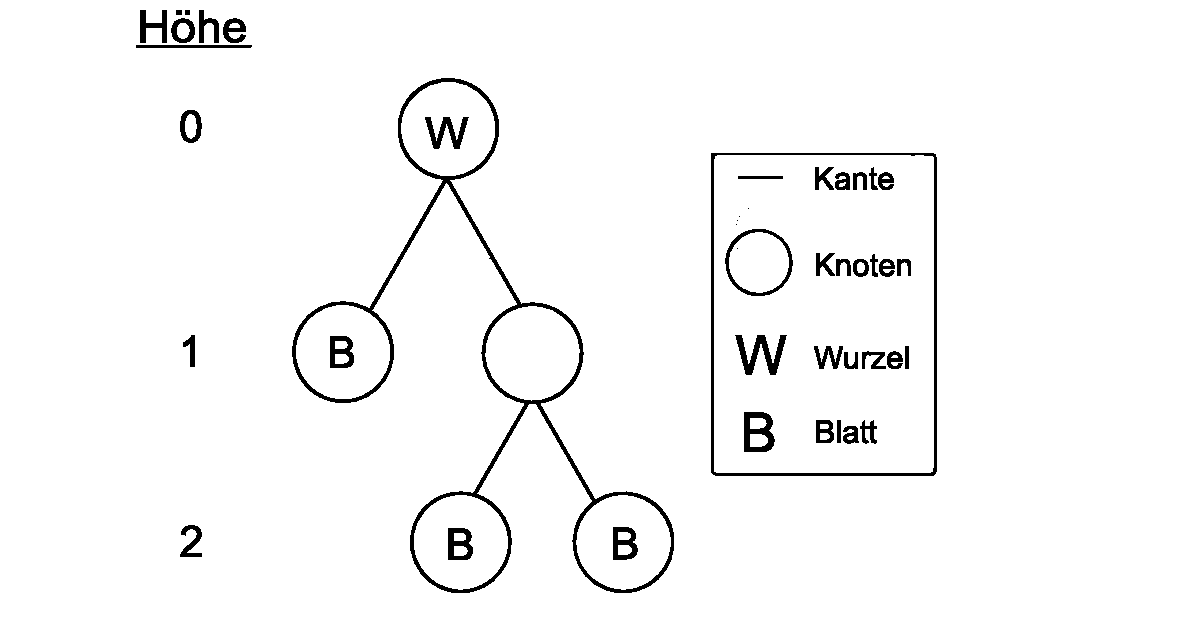
\includegraphics[scale = 0.5]{abbildungen/simple_tree}
    \caption{Einfacher beschrifteter Binärbaum}
    \label{pic:simple_tree} 
\end{figure}

Eine spezielle Form von Bäumen stellen die sogenannten Binärbäume dar. 
Binärbäume sind Bäume, wo jeder Knoten maximal zwei Kinder hat. Abbildung \ref{pic:simple_tree} 
zeigt einen einfachen Binärbaum, wo jedes Element genau beschriftet ist. 

Um jeden Knoten eines Baumes abarbeiten zu können, kann über dem Baum 
traversiert werden. Traversierung bezeichnet das systematische Ablaufen 
von jedem Knoten eines Baumes. Der naive Algorithmus
von Wetherell und Shannon verwendet die sogenannte
Pre-Order-Traversierung. Dabei wird zunächst der Knoten, dann der linke Teilbaum
und zum Schluss der rechte Teilbaum besucht. Hier werden die Väter also vor den
Kindern durchlaufen. Sowohl der verbesserte Algorithmus von Wetherell 
und Shannon als auch der Algorithmus von Reingold und Tilford verwenden hingegen die 
Post-Order-Traversierung. Dabei wird als erstes der linke Teilbaum, dann der 
rechte Teilbaum und dann der Knoten besucht \cite[]{q4}. Bei dieser Art der 
Traversierung werden die Kinder also vor den Väter durchlaufen. Neben diesen Arten
der Traversierung gibt es noch weitere Möglichkeiten, wie über einem 
Baum traversiert werden kann. Diese sind für das Verständnis der hier 
vorgestellten Algorithmen aber nicht notwendig.


\section{Anwendungsgebiete}

Bäume erfahren einen vielfältigen Einsatz in der Informatik, zum Beispiel 
als Datenstruktur, als Syntaxbäume, als Ausdrucksbäume oder auch als 
Entscheidungsbäume.

Ein Baum als Datenstruktur kann beispielsweise dazu verwendet werden, 
um eine Menge von Daten zu sortieren oder in ihnen effizient nach einen 
bestimmten Datensatz zu suchen. So verwendet der Heap-Sort-Algorithmus 
einen Baum zum Sortieren von Daten. Ebenso können Bäume dazu verwendet 
werden, die Syntax von Quellcode zu überprüfen. Ferner werden diese Bäume 
als Syntaxbäume bezeichnet. Zudem werden Bäume verwendet um mathematische 
Ausdrücke auszuwerten. Hierfür wird ein sogenannter Ausdrucksbaum für einen 
gegebenen mathematischen Ausdruck aufgestellt und ausgewertet. In der 
Datenanalyse werden Bäume in Form von Entscheidungsbäumen verwendet. 
Diese werden benutzt um Abhängigkeiten darzustellen. Die Blätter stellen 
Kategorien dar und die Knoten Bedingungen. So können beispielsweise neue 
Datensätze, in Abhängigkeit zu seinen Werten, einer bestimmten Kategorie 
zugeordnet werden.

Auch außerhalb der Informatik werden Bäume häufig verwendet. Sie können 
dazu verwendet werden um zum Beispiel eine Hierarchie eines Unternehmens 
(siehe Abb. 1) dazustellen oder einen Stammbaum einer 
Familie (siehe Abb. 2) \cite[]{q4}.

\todo{Zwei beispielhafte Abbildungen erstellen}


\chapter{Algorithmen zum Zeichnen von Bäumen}
\label{chap:kapitel3}

\section{Naiver Algorithmus von Wetherell und Shannon}

Das Paper “Tidy Drawings of Trees” von Charles Wetherell und Alfred Shannon aus dem Jahre 1979, 
welches im IEEE Trans. Softw. Eng. erschienen ist, handelt von verschiedenen Algorithmen zum Zeichnen von Bäumen.
Der erste Algorithmus, der von den beiden Autoren beschrieben und vorgestellt wird, ist ein naiver Algorithmus 
zum Zeichnen von Bäumen. Dieser Algorithmus soll dabei zwei Anforderungen erfüllen. Die erste Anforderung wird dabei
an die Ästhetik des gezeichneten Baumes gestellt. Alle Knoten, die dieselbe Höhe haben, sollen sich auf einer horizontalen
Linie befinden. Jede Höhe hat dabei eine Linie, auf welcher sich die Knoten befinden sollen und diese Linien sollen alle
parallel zueinander sein. Außerdem soll der Algorithmus beim Zeichnen eines Baumes ein physikalisches Limit einhalten.
Das bedeutet, dass der Algorithmus möglichst schmale Bäume zeichnen soll. Jedoch wird die Höhe des Baumes durch diese Anforderungen
nicht eingeschränkt. Stattdessen bestimmt der Baum selbst seine Höhe. \cite[]{q1}

\subsection{Ablauf}
Bevor die Funktionsweise des Algorithmus beschrieben werden kann, muss die Baumstruktur wie folgt definiert sein: Sie benötigt eine Struktur die symbolisch für ein Knoten des Baums steht. Diese Knoten-Struktur muss hierbei ihren Vater kennen, auf ihre Kinder zugreifen können, ihre Position speichern können. Diese Hilfsvariable wird dazu benutzt, um das nächste abzuarbeitende Kind eines Knoten zu identifizieren. 

In Java könnte diese Struktur beispielsweise wie folgt aussehen:
\begin{lstlisting}
class Knoten {
	Knoten vater;
	Knoten[] kinder;
	int hoehe;
	int x, y;
}
\end{lstlisting}
Dieser Algorithmus besitzt zwei Eingabeparameter: Die Wurzel und Höhe des Baumes. Die Wurzel muss hierbei vom Typ der zuvor definierten Struktur sein. Zu Beginn wird eine Variable definiert: Ein Array (später Positions-Array genannt), die die jeweils nächst freie X-Position einer Ebene des Baums beinhaltet. Hiernach wird über die Baumstruktur der Wurzel, in der Pre-Order-Traversierung, traversiert. Nun werden die X und Y Attribute der Knoten wie folgt bestimmt und gesetzt:

Der derzeitige Knoten bekommt als X-Position den Wert aus dem Positions-Array, in Abhängigkeit von seiner Höhe im Baum. Hiernach wird die Zahl im Positions-Array inkrementiert. Die Y-Position des Knoten wird nun in Abhängigkeit zur Höhe des Knoten mit der folgenden Formel berechnet: y := 2 * Höhe + 1.

Dieses Vorgehen wird nun für alle Knoten in dem Baum wiederholt. 

Nach dem Durchlaufen aller Knoten des Baumes sind alle X und Y-Koordinate gesetzt und der Baum kann gezeichnet werden.

\subsection{Vor- und Nachteile}

\section{Verbesserter Algorithmus von Wetherell und Shannon}

\subsection{Ablauf}

\subsection{Vor- und Nachteile}

\section{Algorithmus von Reingold und Tilford}

\subsection{Ablauf}

\subsection{Implementierung in Java}

\subsection{Vor- und Nachteile}

\subsection{Modifizierung des Algorithmus}


\section{Verbesserter Algorithmus von Wetherell und Shannon}
\label{chap:kapitel3_2}
Wetherell und Shannon stellen in Ihrem Paper einen weiteren, verbesserten Algorithmus zum Zeichnen von Bäumen vor, welcher jedoch
ausschließlich Binärbäume zeichnen kann \cite{q1}. Dieser Algorithmus weist die Nachteile des naiven Algorithmus nicht mehr auf.
Dafür definieren sie zwei weitere Anforderungen, die der Algorithmus erfüllen soll. Jene Anforderungen sind speziell für
die von ihm produzierten Darstellungen von Binärbäume.   

\begin{quotation}
	\textit{Aesthetic 2:} In a binary tree, each left son should be positioned
	left of its father and each right son right of its father \cite[S. 517]{q1}.
\end{quotation}

In einem Binärbaum hat jeder Knoten maximal ein linkes und maximal ein rechtes Kind. Daher soll jedes linke Kind 
links vom Vater und jedes rechte Kind rechts vom Vater positioniert werden. Zudem soll jeder Vater zentriert über seinen Kindern
stehen. Dieses Verhalten legen Wetherell und Shannon in einer weiteren Anforderung fest.

\begin{quotation}
	\textit{Aesthetic 3:} A parent should be centered over its children \cite[S. 518]{q1}.
\end{quotation}

Im Folgenden wird direkt die modifizierte Version des verbesserten Algorithmus betrachtet. Dafür wird die zweite While-Schleife des Programmcodes
mit der Fig. 9 \cite[A modification of Algorithm 3, S. 519]{q1} ersetzt.

\label{chap:kapitel3_2_Ablauf}
\subsection{Ablauf}

Dieser Algorithmus lässt sich in zwei Phasen unterteilen. In der ersten Phase wird die vorläufige X-Koordinate der einzelnen Knoten bestimmt.
In der zweiten Phase werden diese X-Koordinaten bei Bedarf nochmals abgeändert sowie die Y-Koordinate berechnet.

Die Signatur des Algorithmus ist dieselbe wie im naiven Algorithmus. Zu Beginn werden zwei
ganzzahlige Arrays, ein Positions-Array (beinhaltet die nächste freie x-Koordinate auf einer bestimmten Höhe) und ein 
Modifikator-Array (beinhaltet notwendigen Versatz zwischen den Knoten auf einer Höhe), definiert. Diese besitzen die Länge 
\glqq Höhe des Baumes\grqq{}.
Hiernach müssen alle Elemente des Positions-Array mit eins und alle Elemente des Modifikator-Array mit null initialisiert werden.
Zudem wird eine Variable namens \glqq ModifikatorSumme\grqq{} benötigt, welche am Anfang mit null initialisiert wird. Diese Variable wird 
in der zweiten Phase benötigt und speichert alle Modifikatoren von allen Vorgängern eines Knotens.

Durch eine Post-Order-Traversierung werden die vorläufigen x-Koordinaten der Knoten bestimmt.
Dabei wird zwischen vier verschiedenen Fällen unterschieden:
\begin{enumerate}
	\item Der Knoten ist ein Blatt
	\item Der Knoten besitzt kein linkes Kind
	\item Der Knoten besitzt kein rechtes Kind
	\item Der Knoten besitzt sowohl linkes als auch rechtes Kind
\end{enumerate}

Im ersten Fall bekommt der Knoten die nächste freie X-Koordinate auf seiner Höhe. 
Im zweiten Fall wird der Knoten links, mit einem Versatz von eins, von seinem rechten Kind positioniert.
Im dritten Fall wird dieser rechts, mit einem Versatz von eins, von seinem linken Sohn positioniert. Im letzten Fall wird der Knoten
in der Mitte zwischen seinen Kindern positioniert. Hierbei wird die folgende Formel genutzt: $$x = (left.x + right.x) / 2.$$
\todo{Eventuell Gleitkommazahl}
Bei dem zweiten und vierten Fall kann es passieren, dass ein Knoten links von der eigentlich nächsten freien X-Koordinate platziert wird.
Tritt dies ein, so wird das Modifikator-Array angepasst, indem der nötige Versatz auf der Ebene des Knoten auf die Differenz zwischen
der vorläufigen X-Koordinate und der eigentlich nächsten freien X-Koordinate gesetzt wird. Außerdem merkt sich jeder Knoten den Modifikator
auf seiner Höhe, was im zweiten Teil des Algorithmus benötigt wird. Sollte dieser Knoten zudem kein Blatt sein, dann
wird seine vorläufige X-Koordinate nochmal abgeändert. Diese wird dann mit dem Versatz aus dem Array auf seiner Höhe addiert, also nach rechts
verschoben. Zum Schluss wird die nächste freie X-Koordinate auf der Ebene bestimmt. Dafür wird die X-Koordinate des Knoten um einen 
bestimmten Wert addiert (hier zwei) und in das Positions-Array (Index: Höhe des Knotens) geschrieben.

In der zweiten Phase wird zu Beginn eine Variable namens \glqq ModifikatorSumme\grqq{} deklariert und mit null initialisiert. 
Die ModifikatorSumme entspricht der Summe aus allen Modifikatoren der Vorgänger eines Knotens. Um diese Summe zu berechnen, 
wird bei dem Besuch eines Kind-Knotens der spezifische Modifikator des Vaters auf die Summe addiert. Beim Übergang eines Kindes 
zurück auf den Vater wird entsprechend der knotenspezifische Modifikator von der globalen ModifikatorSumme abgezogen.

Da die Pre-Order Traversierung vorgibt, erst den linken Teilbaum, dann den Knoten und zum Schluss den rechten Teilbaum zu besuchen,
wird zunächst beginnend von der Wurzel aus, der am weitesten links unten stehende Knoten besucht. Abbildung \ref{pic:baum_algo_2}
zeigt einen Baum, welcher mit dem verbesserten Algorithmus gezeichnet wurde. In diesem Beispiel wird bei der Wurzel gestartet 
und nach Knoten D gelaufen. Auf dem Weg dorthin werden die Modifikatoren von A und B auf die globale ModifikatorSumme addiert.
Danach wird die X-Koordinate des Knotens entweder auf die nächste freie X-Koordinate auf der Höhe des Knotens gesetzt oder auf den
Wert der vorläufigen X-Koordinate addiert mit der ModifikatorSumme. Dabei wird der kleinere der beiden Werte genutzt, um sicherzustellen,
dass der Knoten möglichst weit links ist. Wenn der Knoten einen linken Sohn hat und die X-Koordinate des Sohnes größer ist als
die X-Koordinate des Vaters, dann wird die X-Koordinate des Vaters auf die X-Koordinate des Sohnes plus eins gesetzt. 
Damit wird sichergestellt, dass der Knoten nicht direkt über seinem linken Sohn steht, sondern eine Position weiter rechts.
Falls der Knoten nicht die Wurzel ist, der Vater des Knotens bereits besucht und abgearbeitet wurde und die X-Koordinate des Knotens
kleiner als die X-Koordinate des Vaters plus eins ist, dann wird die X-Koordinate des Knotens auf die X-Koordinate des Vaters plus eins gesetzt.
Ähnlich wie im Fall vorher dient diese Überprüfung dazu, den Knoten richtig zu positionieren. Hier wird dadurch verhindert,
dass der Knoten genau unter seinem Vater steht. Stattdessen wird sichergestellt, dass der Knoten rechts von seinem Vater steht,
welcher der rechte Sohn sein muss, da der Vater bereits besucht und positioniert wurde. 
Nun ist die X-Koordinate des Knotens final bestimmt worden. Die Y-Koordinate wird genau wie im naiven Algorithmus bestimmt, 
indem die Höhe des Knotens mit zwei multipliziert und mit einem Versatz (hier eins) addiert wird. Zum Schluss wird die nächste 
freie X-Position auf der Höhe des Knotens bestimmt, indem die X-Koordinate mit einem Versatz (hier zwei) addiert wird. 


\subsection{Implementierung in Java}

\begin{figure}[H]
    \centering
    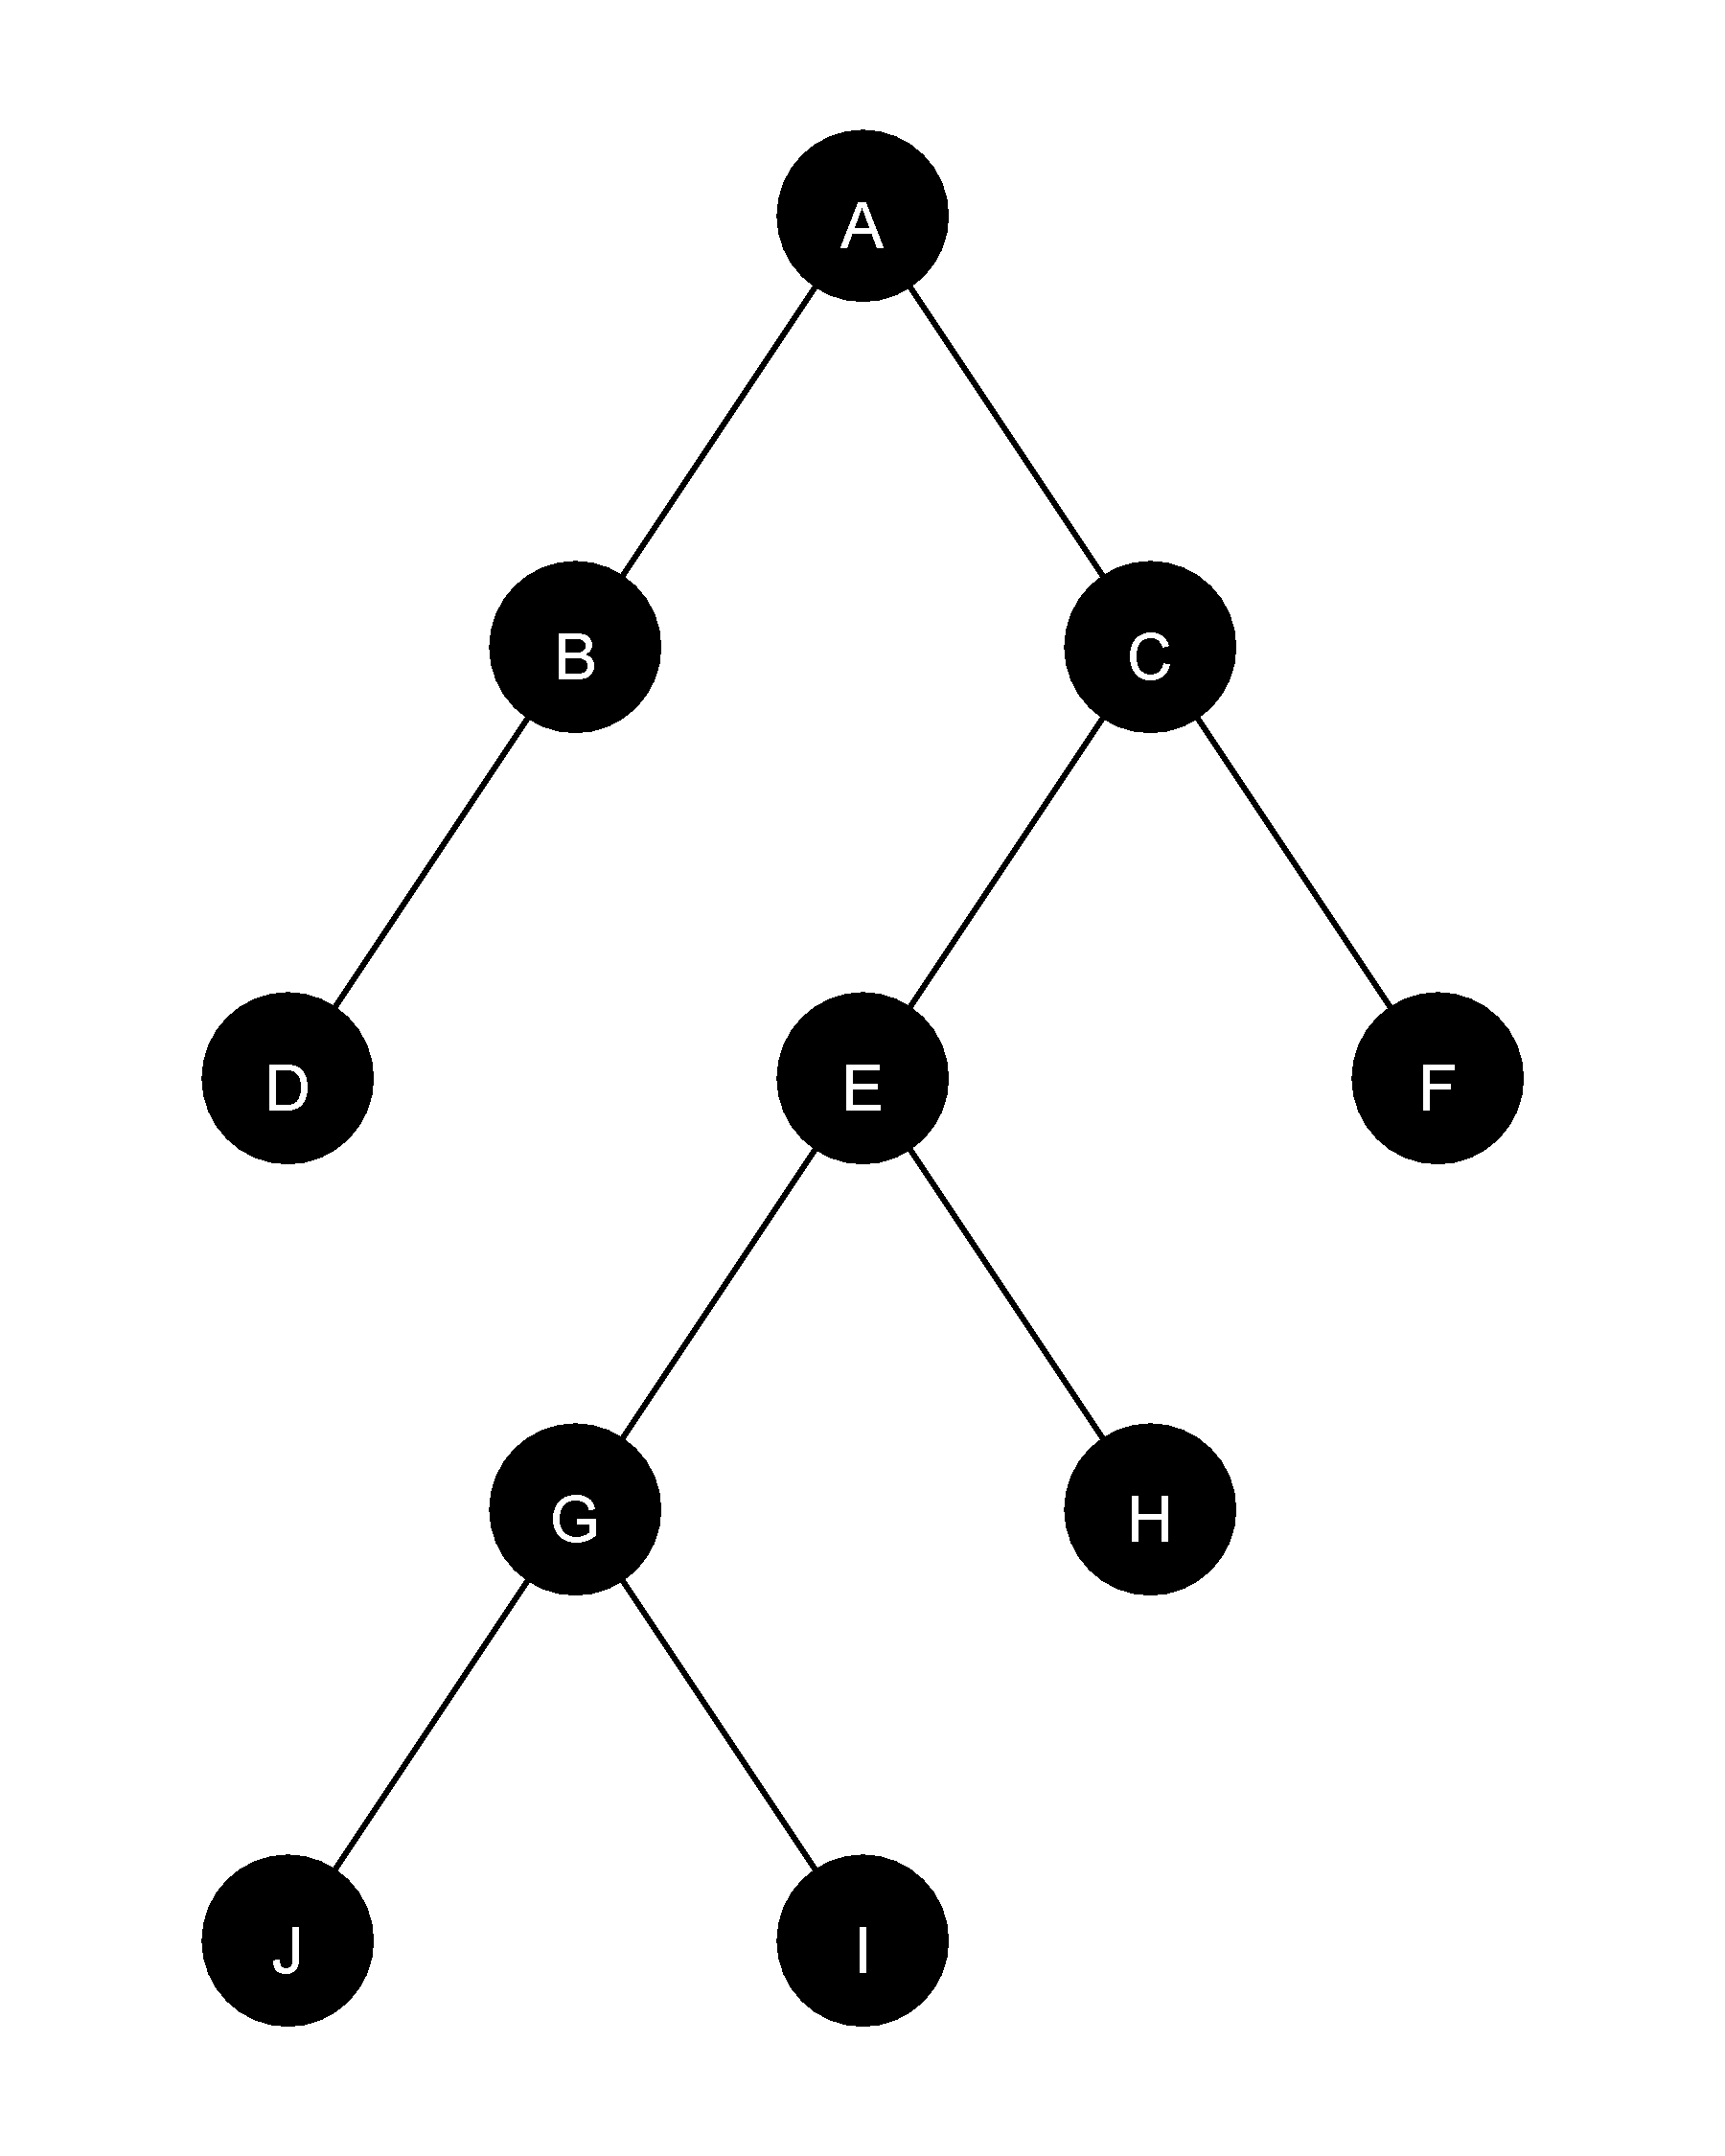
\includegraphics[scale = 0.10]{abbildungen/baum_algo_2}
    \caption{Gezeichneter Baum durch den verbesserten Algorithmus}
    \label{pic:baum_algo_2} 
\end{figure}

Dieser Algorithmus wurde wie der erste Algorithmus in Java implementiert. Da der gezeigte Algorithmus
am Beispiel von Binärbäumen gezeigt wird, wurde eine Binäre-Knoten-Klasse implemeniert,
die von der Knoten-Klasse, gezeigt im Quellcode \ref{code:knotenclass}, erbt. In dieser Klasse wurden
Hilfsmethoden und zwei weitere Attribute definiert. Die Implementierung sieht vereinfacht wie folgt aus:

\begin{lstlisting}[caption=Vereinfachte Implementierung der BinaryKnoten-Klasse, label=code:binaryknotenclass]
public class BinaryKnoten extends Knoten {
    private int modifier;
	private int vistStatus;

    @Override
	public void traversPostOrder(Consumer<Knoten> cons) { 
        // ...
    }

    public BinaryKnoten getLeft() { /*...*/ }
    public BinaryKnoten getRight() { /*...*/ }

    // Getter / Setter ...
}
\end{lstlisting}

Als erstes wurde eine Prozedur mit dem Namen \glqq algorithmus2Verbessert\grqq{} 
definiert, die zwei Eingabeparameter besitzt: der Wurzelknoten des Baums 
und die Höhe des Baums. Zu Anfang werden alle Arrays und Variablen, wie im Ablauf 
bereits beschrieben, initialisiert. Hiernach wird erstmalig in der Post-Order über 
die Baum-Struktur rekursiv traversiert. Hierfür wird die in der Binären-Knoten-Klasse 
zuvor erstellte Methode \glqq traversPostOrder\grqq{} genutzt. Diese übernimmt als Argument einen Consumer, 
in dem die einzelnen Knoten in der geforderten Reihenfolge übergeben werden. In dem übergebenem Consumer 
wird ferner die X-Koordinate und der Modifikator jedes einzelnen Knoten bestimmt.

\begin{lstlisting}[caption=Vereinfachte Implementierung der Phase 1, label=code:algo2_phase1]
wurzel.traversPostOrder(k -> {
    BinaryKnoten knoten = (BinaryKnoten) k;

    // Position / Modifikator des Knoten bestimmen ...
});
\end{lstlisting}

Die zweite Phase wurde so implementiert, dass iterativ über den Baum in der Pre-Order traversiert 
wird. Die Implementierung entspricht dem zuvor gezeigten Ablauf in Kapitel \ref{chap:kapitel3_2_Ablauf}. 

Wird diese Implementierung auf einen beispielhaften Baum angewendet, so kann das Ergebnis
in der Abbildung \ref{pic:baum_algo_2} betrachtet werden.

\subsection{Vor- und Nachteile}
Durch das Erfüllen der Anforderung, dass jeder Vater über seinen Kindern zentriert werden soll, kann der Algorithmus gegen
die Anforderung an das physikalische Limit verstoßen. 
Abbildung \ref{pic:baum_theorem_uglification} zeigt jenes Verhalten. Daraus schließen die beiden Autoren auf folgendes Theorem:

\begin{quotation}
	\textit{Theorem (Uglification):} Minimum width drawings exist which violate Aesthetic 3 by arbitrary amounts \cite[S. 519]{q1}.
\end{quotation}

\begin{figure}[H]
    \centering
    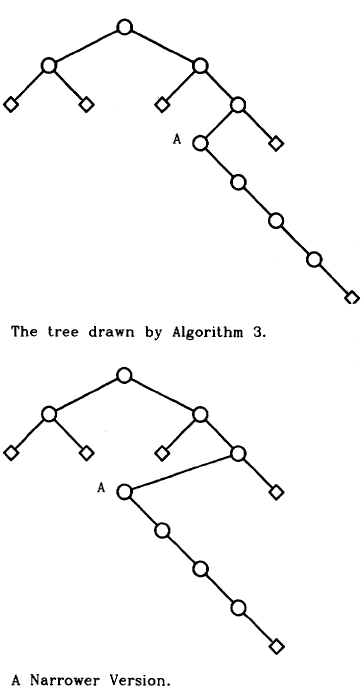
\includegraphics[scale = 0.75]{abbildungen/baum_theorem_uglification}
    \caption{Beispiel für das Theorem \cite[S. 519]{q1}}
    \label{pic:baum_theorem_uglification} 
\end{figure}

Bei der schmaleren Variante des Baumes auf Abbildung \ref{pic:baum_theorem_uglification} ist der Vater von Knoten A nicht zentriert
über beiden Kindern und verstößt somit gegen Aesthetic 3. Die weitere Variante verstößt gegen das physikalische Limit, da der Baum nicht
maximal schmal ist. Dies stellt hier einen Trade-off zwischen den beiden Anforderungen dar. Es ist somit notwendig, dass maximal schmale Bäume der
Anforderungen Aesthetic 3 widersprechen können. 

Im Vergleich zu dem naiven Algorithmus von Wetherell und Shannon zeichnet der verbesserte Algorithmus die Bäume nicht mehr maximal links.
Dies sorgt dafür, dass die gezeichneten Bäume übersichtlicher wirken und ästhetisch ansprechender sind. Falls die Knoten einen Inhalt haben, dann
ist die Positionierung der Knoten auch von Relevanz, da das linke Kind kleiner und das rechte Kind größer als der Knoten ist. Beispielsweise
Suchbäume sind dadurch auch intuitiver zu verstehen, da die Größe des Inhalts von links nach rechts aufsteigend sortiert ist. 

Zudem ist der verbesserte Algorithmus typischerweise nicht in der Lage beliebige Bäume zu zeichnen, sondern ausschließlich Binärbäume.


\label{chap:kapitel3_3}
\section{Algorithmus von Reingold und Tilford}

Das Paper \glqq Tidier Drawings of Trees\grqq{} von Edward M. Reingold und John S. Tilford aus dem Jahre 1981,
welches im IEEE Transaction on Software Engineering erschienen ist, handelt von einem Algorithmus zum Zeichnen von Bäumen im Ebenen-Layout\cite[]{q2}.
Die Motivation der beiden Autoren für das Erstellen dieses Algorithmus beruht darauf, dass sie ein entscheidendes Problem an dem 
verbesserten Algorithmus von Wetherell und Shannon erkannt haben. Dieser Algorithmus ohne die Modifikation produziert Bäume, 
welche nicht maximal schmal sind, da das Zentrieren der Väter erzwungen wird. Die modifizierte Variante des 
Algorithmus produziert zwar maximal schmale Bäume, dafür können diese wesentlich unübersichtlicher sein, 
was der untere Baum auf Abbildung \ref{pic:baum_theorem_uglification} zeigt\footnote[1]{In dieser Arbeit wurde lediglich die modifizierte Variante
vorgestellt, siehe \ref{chap:kapitel3_2}.}. 
Reingold und Tilford erkennen, dass das Problem an dem Algorithmus ist, dass die einzelnen Teilbäume von Knoten außerhalb des Teilbäume 
beeinflusst werden. Daraus folgern die beiden, dass es mit dem Algorithmus von Wetherell und Shannon dazu kommen kann, dass ein Baum und 
die Spiegelung desselben Baumes keine Spiegelbilder ergeben. Jedoch wäre es nach Reingold und Tilford wünschenswert, wenn symmetrische Bäume 
auch symmetrisch gezeichnet werden. Daraus wird eine weitere Anforderung an Algorithmen zum Zeichnen von Bäumen abgeleitet \cite[S.224]{q2}.

\begin{quotation}
	\textit{Aesthetic 4:} A tree and its mirror image should produce
    drawings that are reflections of one another; moreover, a subtree
    should be drawn the same way regardless of where it
    occurs in the tree \cite[S.224]{q4}.
\end{quotation}

Wenn der Algorithmus eine Spiegelung eines Baumes erhält und der durch den Algorithmus gezeichnete Baum ein exaktes Spiegelbild des 
eigentlichen Baumes ist, dann ist diese Anforderung erfüllt. Abbildung \ref{pic:WS_Spiegel} zeigt einen Baum und seine Spiegelung der mit 
unserer Implementierung des Algorithmus von Wetherell und Shannon gezeichnet wurde. Abbildung \ref{pic:TR_Spiegel} zeigt den selben Baum mit 
seiner Spiegelung, aber dieses mal mit unserer Java-Implementierung von Reingold und Tilfords Algorithmus. Zu erkennen an dieser Abbildung ist, 
dass der Algorithmus von Reingold und Tilford Aesthetic 4 erfüllt, der Algorithmus von Wetherell und Shannon jedoch nicht. Außerdem sollen 
Teilbäume immer gleich gezeichnet werden, unabhängig von ihrer Position im Baum.

Um diese Anforderung zu erfüllen, dürfen Knoten außerhalb eines Teilbaums die Knoten innerhalb eines Teilbaums nicht beeinflussen. 
Damit das erreicht wird, werden bei diesem Algorithmus nicht einzelne Knoten platziert (wie bei Wetherell und Shannon), 
sondern es werden zwei Teilbäume unabhängig voneinander betrachtet und dann so nah wie möglich aneinander platziert \cite[S.225]{q2}. 

\label{chap:kapitel3_3_Ablauf}
\subsection{Ablauf}

\begin{figure}[ht]
    \centering
    \begin{minipage}[]{0.3\linewidth}
        \centering
        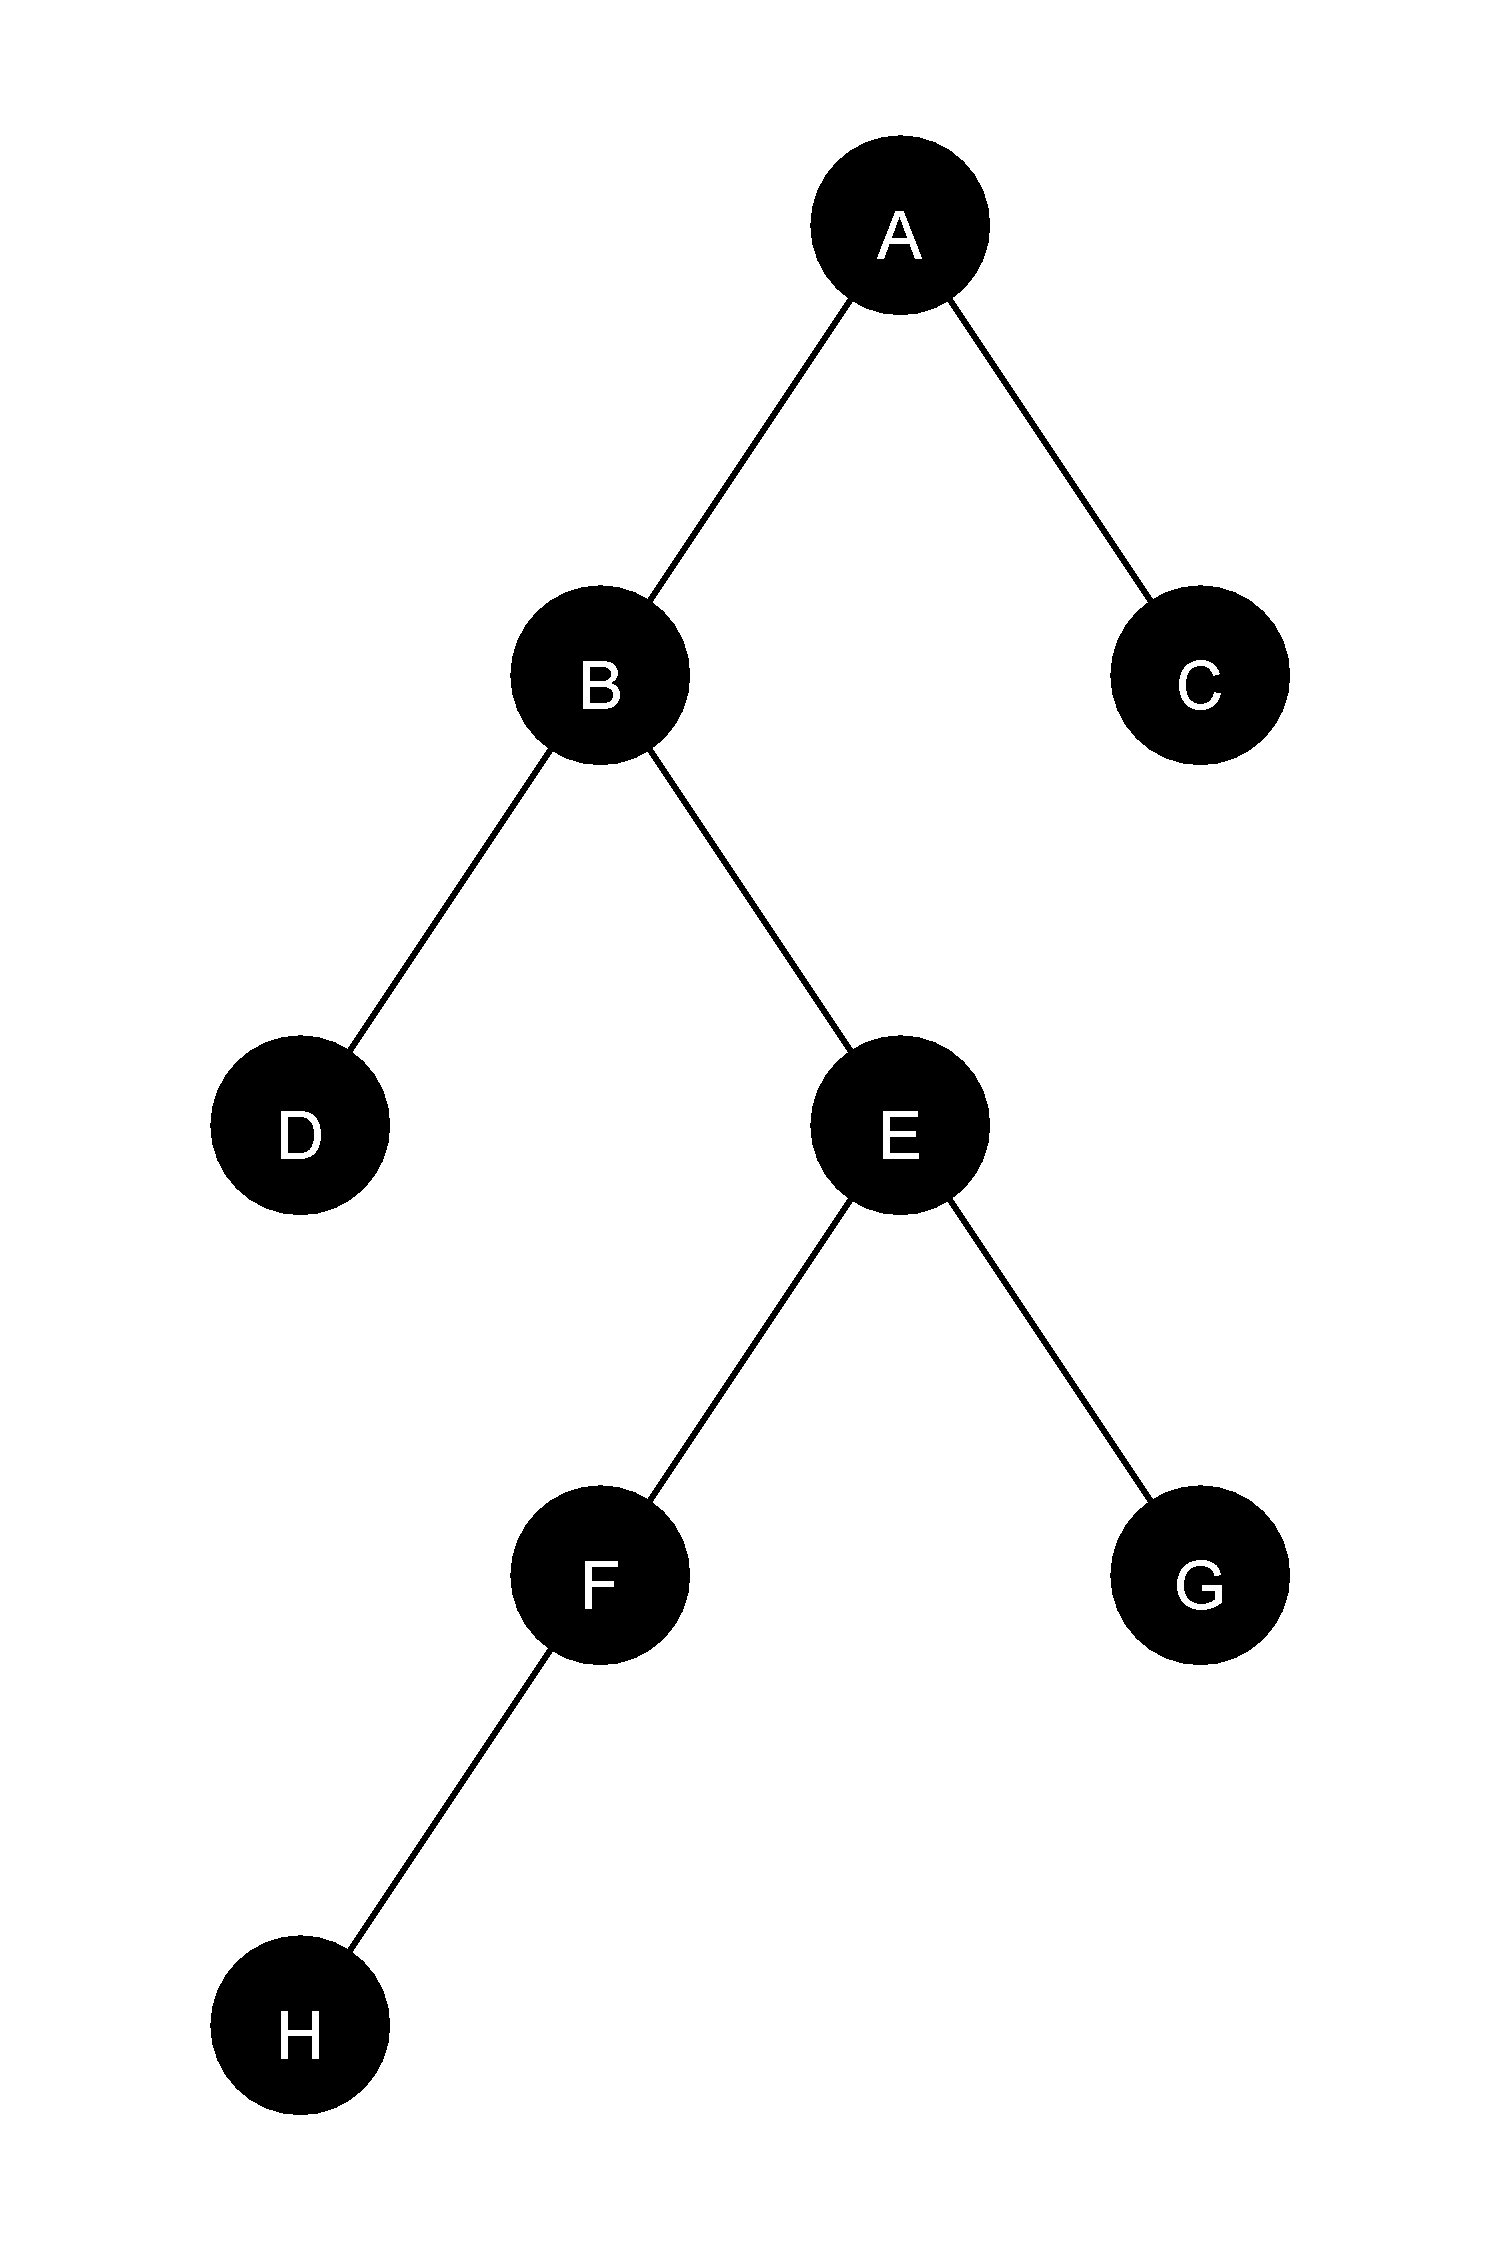
\includegraphics[scale=0.07]{abbildungen/tree_beispiel_LL_LR_RL_RR}
    \end{minipage}
    \hfill
    \begin{minipage}[]{0.65\linewidth}
        \centering
        \begin{tabular}{l | c | c | c | c | c | c | c | c}
            & A & B & C & D & E & F & G & H \\
            \hline\hline
            \textbf{LL} & H & D & C & D & H & H & G & H \\
            \textbf{LR} & G & D & C & D & F & H & G & H \\
            \textbf{RL} & C & H & C & D & G & H & G & H \\
            \textbf{RR} & C & G & C & D & G & H & G & H \\
            \end{tabular}
    \end{minipage} 
    \caption{Beispielhafte Bestimmung für LL, LR, RL, RR}
\end{figure}

Der Algorithmus zum Zeichnen von Bäumen von Reingold und Tilford lässt sich in zwei Phasen unterteilen.
Den ersten Teil stellt die Prozedur “Setup” dar. Diese Prozedur erhält vier Eingabeparameter, nämlich einen Knoten (welche am Anfang 
die Wurzel ist), die Höhe des Knotens im Gesamtbaum, sowie RMOST und LMOST. RMOST und LMOST sind jedoch nicht vom Datentyp Knoten, sondern 
von einem neuen Datentyp namens Extreme. Extreme sind Strukturen, die drei Attribute besitzen: 
\begin{itemize}
    \item Verweis auf einen Knoten
    \item Offset von der X-Koordinate zur Wurzel des Teilbaums
    \item Höhe des Knotens im Gesamtbaum
\end{itemize}

Zu Beginn der Prozedur wird geprüft, ob der übergebene Knoten NULL ist. Wenn dies nicht der Fall ist, 
dann wird die Y-Koordinate des Knotens auf seine Höhe gesetzt. Danach wird die Prozedur rekursiv aufgerufen, 
um eine Post-Order Traversierung auszuführen. Dieser Aufruf sieht wie folgt aus:

\begin{lstlisting}[caption = Rekursiver Aufruf von Setup]
    SETUP (L, LEVEL+1, LR, LL );
    SETUP (R, LEVEL+1, RR, RL );
\end{lstlisting}

Durch die Post-Order Traversierung wird die Setup Prozedur solange aufgerufen, bis der aktuelle Knoten das Blatt unten links ist. 
Da ein Blatt automatisch der am weitesten links und am weitesten rechts stehende Knoten ist, werden die Adressen von 
RMOST und LMOST auf diesen Knoten gesetzt. Außerdem wird die Höhe von RMOST und LMOST auf die Höhe des aktuellen Knotens gesetzt. 
Zudem werden die Offsets des Knotens und von RMOST sowie LMOST auf null gesetzt. 

Wenn der Knoten sowohl ein linkes als auch ein rechtes Kind hat, dann wird geprüft, ob das linke Kind ein rechtes Kind hat. 
Ist dies der Fall, dann wird der Offset des linken Kindes auf die Summe der linken Offsets addiert und vom aktuellen Abstand abgezogen. 
Zudem wird dann der Zeiger auf das linke Kind auf das rechte Kind des linken Kindes gesetzt. Andernfalls, wird dann der Offset des linken 
Kindes von der Summe der linken Offsets subtrahiert und der aktuelle Abstand um den Offset des linken Kindes erhöht. Auch wird danach der 
Zeiger auf das linke Kind auf das linke Kind des linken Kindes gesetzt. Genau dasselbe wird auch für das rechte Kind geprüft und ausgeführt. 
Falls danach der aktuelle Abstand kleiner als ein vorher festgelegter Mindestabstand ist, wird der Abstand zwischen den Kindern um den 
Mindestabstand minus dem aktuellen Abstand erhöht. Außerdem wird der aktuelle Abstand dann auf den Mindestabstand gesetzt. Dies wird solange 
ausgeführt, bis einer der beiden Zeiger (auf linkes/rechtes Kind) gleich NULL ist. Diese Schleife sorgt dafür, dass entlang der rechten 
Kontur des linken Teilbaums und entlang der linken Kontur des rechten Teilbaums die Distanz zwischen den beiden bestimmt wird. 
Gegebenenfalls werden dann die beiden Teilbäume auseinander geschoben, falls sie sich berühren \cite[S.226]{q2}.

Nach dieser Schleife wird der Offset des aktuellen Knotens auf die Hälfte des Abstandes zwischen den Kindern plus eins gesetzt. 
Dieser Offset wird dann von der Summe der linken Offsets abgezogen und auf die Summe der rechten Offsets addiert. 

Danach werden RMOST und LMOST mit Hilfe von \ac{LL}, \ac{LR}, \ac{RL} und \ac{RR} neu festgelegt. Wenn die Höhe von \ac{RL} größer als die Höhe von \ac{LL} ist oder 
der aktuelle Knoten kein linkes Kind hat, dann setze LMOST auf \ac{RL} und erhöhe den Offset von LMOST um den Offset des Knotens. 
Ansonsten setze LMOST auf \ac{LL} und ziehe vom Offset von LMOST den Offset des Knotens ab. Diese Abfrage wird für RMOST und \ac{LR} sowie \ac{RR} 
wiederholt. Es wird geprüft, ob die Höhe von \ac{LR} größer ist als die Höhe von \ac{RR} oder der Knoten kein rechtes Kind hat. Wenn dies der Fall ist, 
dann wird RMOST auf \ac{LR} gesetzt und der Offset von RMOST um den Offset des Knotens verringert. Tritt dieser Fall nicht ein, dann wird RMOST 
auf \ac{RR} gesetzt und der Offset von RMOST mit dem Offset des Knotens addiert. 

RMOST und LMOST korrekt festzulegen ist für den nächsten Schritt wichtig und notwendig. Diese beiden Knoten in einem Subtree 
sind die einzigen, bei denen die Möglichkeit besteht, dass Threading angewandt wird. Threads sind eine Art \glqq Pseudo-Kante \grqq{}, 
welche eingefügt werden, um sicherzustellen, dass sich zwei Teilbäume nicht berühren. Jene Hilfe ist speziell für diesen Algorithmus
und findet in den anderen Algorithmen keine Anwendung. Dieser Schritt ist nur dann nötig, wenn 
die beiden betrachteten Teilbäume eines Knotens unterschiedlich hoch sind und keiner von beiden leer ist. Reingold und Tilford 
geben dafür ein Beispiel an. Wenn der linke Subtree höher als der rechte Subtree ist, dann muss ein Thread von \ac{RR} zu dem am weitesten 
rechts stehenden Knoten des linken Teilbaums auf der nächsten Höhe gelegt werden. Dieser Thread würde in dem Zeiger auf das linke Kind 
von \ac{RR} gespeichert werden \cite[S.226]{q2}.

Die zweite Phase des Algorithmus stellt die Prozedur “petrify” dar. Ziel dieser Prozedur ist es die relativen Offsets, 
welche in der vorherigen Phase gesetzt worden, in absolute Koordinaten umzuwandeln. Zudem sorgt die Prozedur dafür, dass die Threads 
gelöscht werden, da diese nicht mehr benötigt werden. Um dies zu erreichen wird eine Pre-Order-Traversierung 
über dem Baum durchgeführt. Dafür bekommt “petrify” zwei Eingabeparameter, nämlich einen Knoten (zu Beginn wieder die Wurzel) und eine 
initiale X-Position (ist beliebig). Dann prüft die Prozedur, ob der Knoten ungleich NULL ist. Wenn dies der Fall ist, dann wird geschaut, 
ob der Knoten einen Thread hat. Da Threads Blätter sein müssen, werden die Verweise des Knotens auf sein linkes und rechtes Kind gelöscht, 
um keinen Thread fälschlicherweise als Kante darzustellen. Dann setzt die Prozedur die finale X-Koordinate des Knotens auf den 
übergebenen Parameter. Zum Schluss wird “petrify” wie folgt rekursiv aufgerufen:

\begin{lstlisting}[caption=Rekursiver Aufruf von Petrify (Pre-Order)]
    PETRIFY(T.LLINK, XPOS - T.OFFSET);
    PETRIFY(T.RLINK, XPOS + T.OFFSET);
\end{lstlisting}

Bei linken Kindern wird der Offset des Vaters von der X-Koordinate abgezogen. Bei rechten Kindern wird dann die X-Koordinate mit dem 
Offset des Vaters addiert. Ziel dessen ist, dass linke Kind links vom Vater und rechte Kinder rechts vom Vater stehen.


\subsection{Implementierung in Java}

\begin{figure}[H]
    \centering
    
\includegraphics[scale = 0.05]{abbildungen/baum_algo_3_n1}
    \caption{Gezeichneter komplexer Baum durch den Tilford Algorithmus}
    \label{pic:baum_algo_3_n1} 
\end{figure}

\begin{figure}[H]
    \centering
    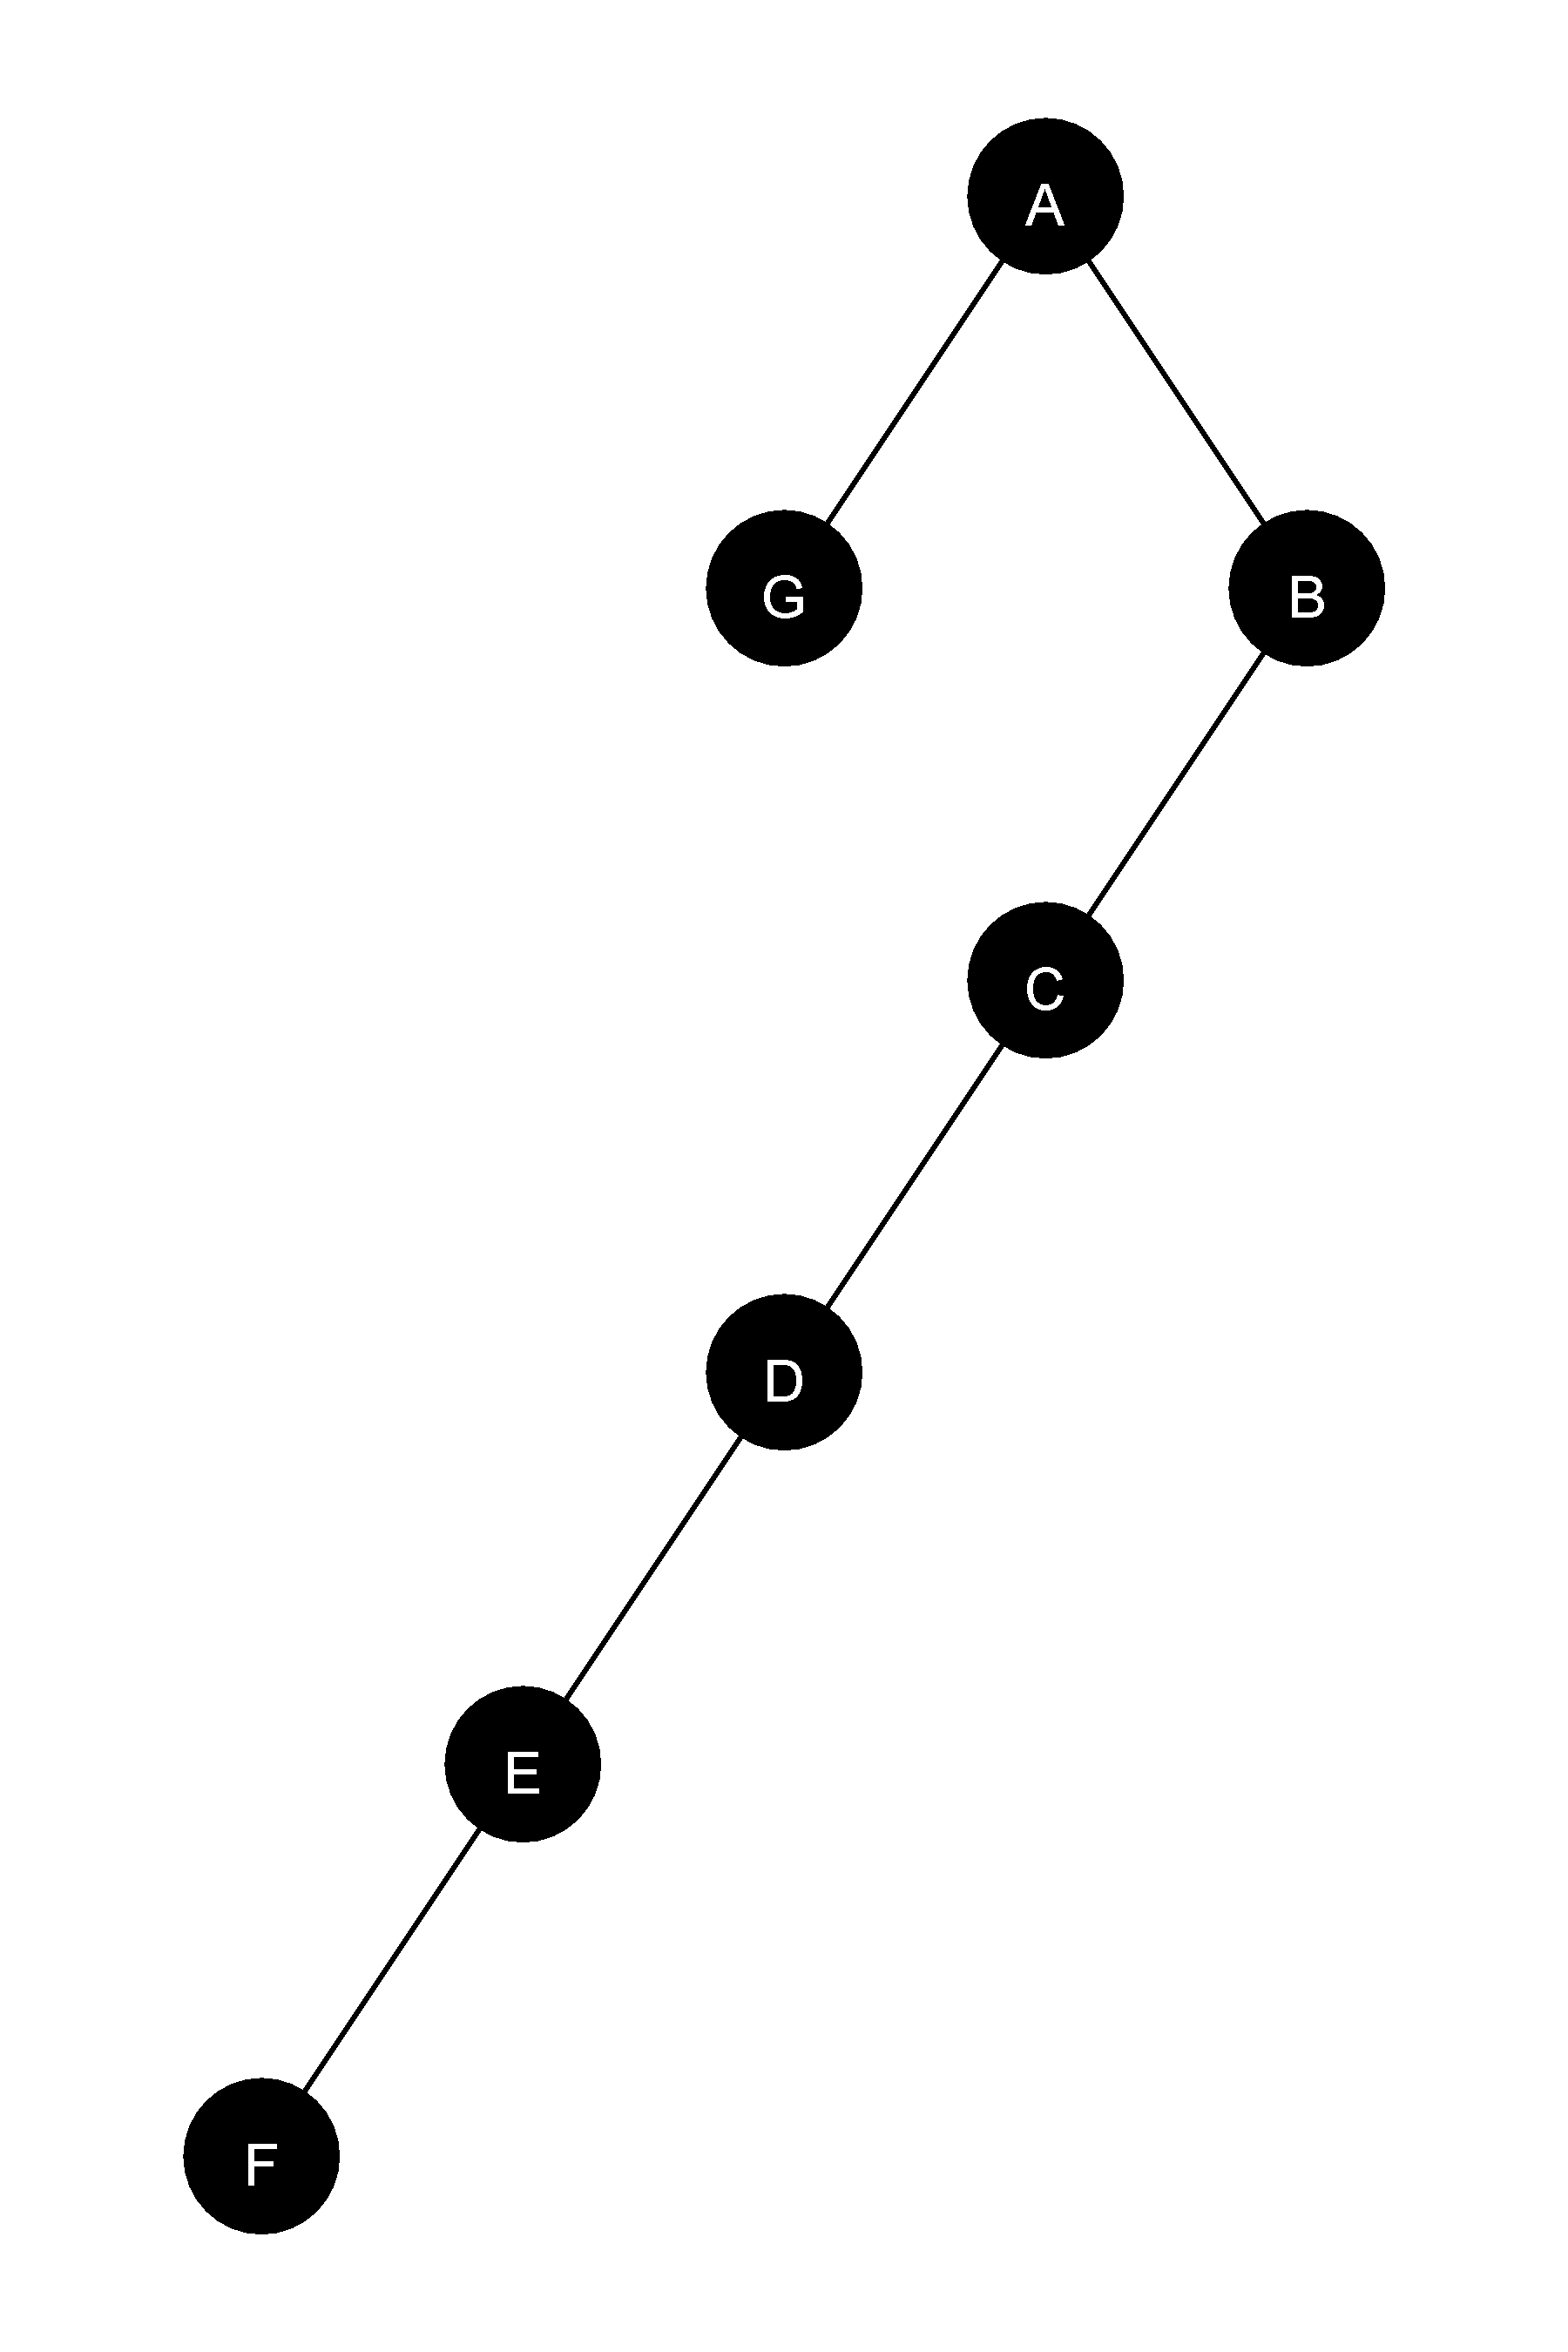
\includegraphics[scale = 0.07]{abbildungen/baum_algo_3_n2}
    \caption{Gezeichneter einfacher Baum durch den Tilford Algorithmus}
    \label{pic:baum_algo_3_n2} 
\end{figure}

Um diesen Algorithmus implementieren zu können, muss die zuvor erstellte BinaryKnoten-Klasse um ein 
Attribut erweitert werden: vom Typ Boolean mit dem Namen \glqq thread\grqq{}. Zudem wurde eine weitere Klasse 
namens \glqq Extreme\grqq{} definiert, die wie zuvor beschrieben, implementiert wurde. Die Extreme-Klasse sieht wie folgt aus:

\begin{lstlisting}[caption=Implementierung der Extreme-Klasse, label=code:algo3_extreme]
private static class Extreme {
    BinaryKnoten knoten;
    int offset;
    int level;
    
    void set(BinaryKnoten k, int offset) {
        this.knoten = k;
        this.level = k.getHoehe();
        this.offset = offset;
    }
}
\end{lstlisting}

Ferner wurden die zuvor beschriebenen Prozeduren \glqq setup\grqq{} und \glqq petrify\grqq{} implementiert. Die implementierte Prozedur
\glqq setup\grqq{} unterscheidet sich zum zuvor beschriebenen Ablauf. Sie wird nun nicht mehr rekursiv aufgerufen und besitzt 
nur einen Eingabeparameter, den Wurzelknoten. Hiernach wird mithilfe der \glqq traversPostOrder\grqq{}-Methode aus der 
BinaryKnoten-Klasse über den Baum traversiert.

\begin{lstlisting}[caption=Ausschnitt aus der setup-Prozedur, label=code:algo3_setup]
public static void setup(BinaryKnoten wurzel) {
    // Initialisierungen von Variablen
    // <...>
    // Ueber den Baum in der Post-Order traversieren
    wurzel.traversPostOrder(k -> {
        BinaryKnoten knoten = (BinaryKnoten) k;

        // Bestimmen der Y-Koordinate
        knoten.setY(2 * knoten.getHoehe() + 1);

        // Vorlaeufige relative X-Koordinate bestimmem
        // <...>
    }
}
\end{lstlisting}

Abweichend zum Ablauf entspricht die Y-Koordinate nicht der Höhe des Knotens. Stattdessen wird diese wie im 
Ablauf aus dem Kapitel \ref{chap:kapitel3_1_Ablauf} berechnet. Dies bietet den Vorteil, 
dass die Methodik zum Zeichnen der Bäume nicht verändert werden muss. Die weitere Implementierung folgt 
der Beschreibung aus dem Ablauf.

Die Implementierung der Prozedur \glqq petrify\grqq{} entspricht der Beschreibung aus dem Ablauf.

Hiernach wurde die Prozedur \glqq algorithmus3\grqq{} definiert. Diese ruft zu Beginn die beiden Prozeduren, 
\glqq setup\grqq{} und \glqq petrify\grqq{} auf. Danach müssen die X-Koordinaten noch angepasst werden, da diese 
negativ sein können. Hierfür wird der kleinste X-Wert ermittelt, dessen absoluter Wert 
addiert mit eins in der Variable \glqq offset\grqq{} gespeichert wird. Nun werden alle X-Koordinaten des 
Baums mit dem Wert aus \glqq offset\grqq{} addiert. 

Zwei beispielhafte Ergebnisse können in den Abbildungen \ref{pic:baum_algo_3_n1} 
und \ref{pic:baum_algo_3_n2} betrachtet werden. 


\subsection{Vor- und Nachteile}

Ein Algorithmus, welcher Aesthetic 4 erfüllt, kann Bäume produzieren, welche nicht maximal schmal sind. 
Für Reingold und Tilford ist das Erfüllen dieser Anforderung jedoch wichtiger als das Einhalten des physikalischen Limits, 
da Aesthetic 4 dafür sorgt, dass diese Bäume für Menschen übersichtlicher und leichter zu verstehen sind \cite[S.224]{q2}. Dafür ist der Algorithmus 
jedoch, gemessen an den Zeilen im Programmcode, der längste. Selbst bei komplexeren Bäumen, wie in Abbildung \ref{pic:baum_algo_3_n2},
wird ein übersichtlicher und ästhetisch ansprechender Baum gezeichnet. 

Ähnlich wie der verbesserte Algorithmus von Wetherell und Shannon ist der Algorithmus von Reingold und Tilford so wie er ist nur in Lage
Binärbäume zu zeichnen. Jedoch beschreiben die beiden Autoren wie der Algorithmus modifiziert werden kann um beliebige Bäume zu zeichnen.



% ***************************** BIBLIOGRAPHY **********************************
\baselineskip=14pt
\clearpage
\phantomsection
\addcontentsline{toc}{chapter}{\protect\numberline{}\bibname}
\bibliography{bib/thesis}

% ******************************* APPENDIX ************************************
\appendix
\chapter{Anhang A}
\label{chap:anhang_a}

\begin{figure}[ht]
    \centering
    \begin{minipage}[t]{0.45\linewidth}
        \centering
        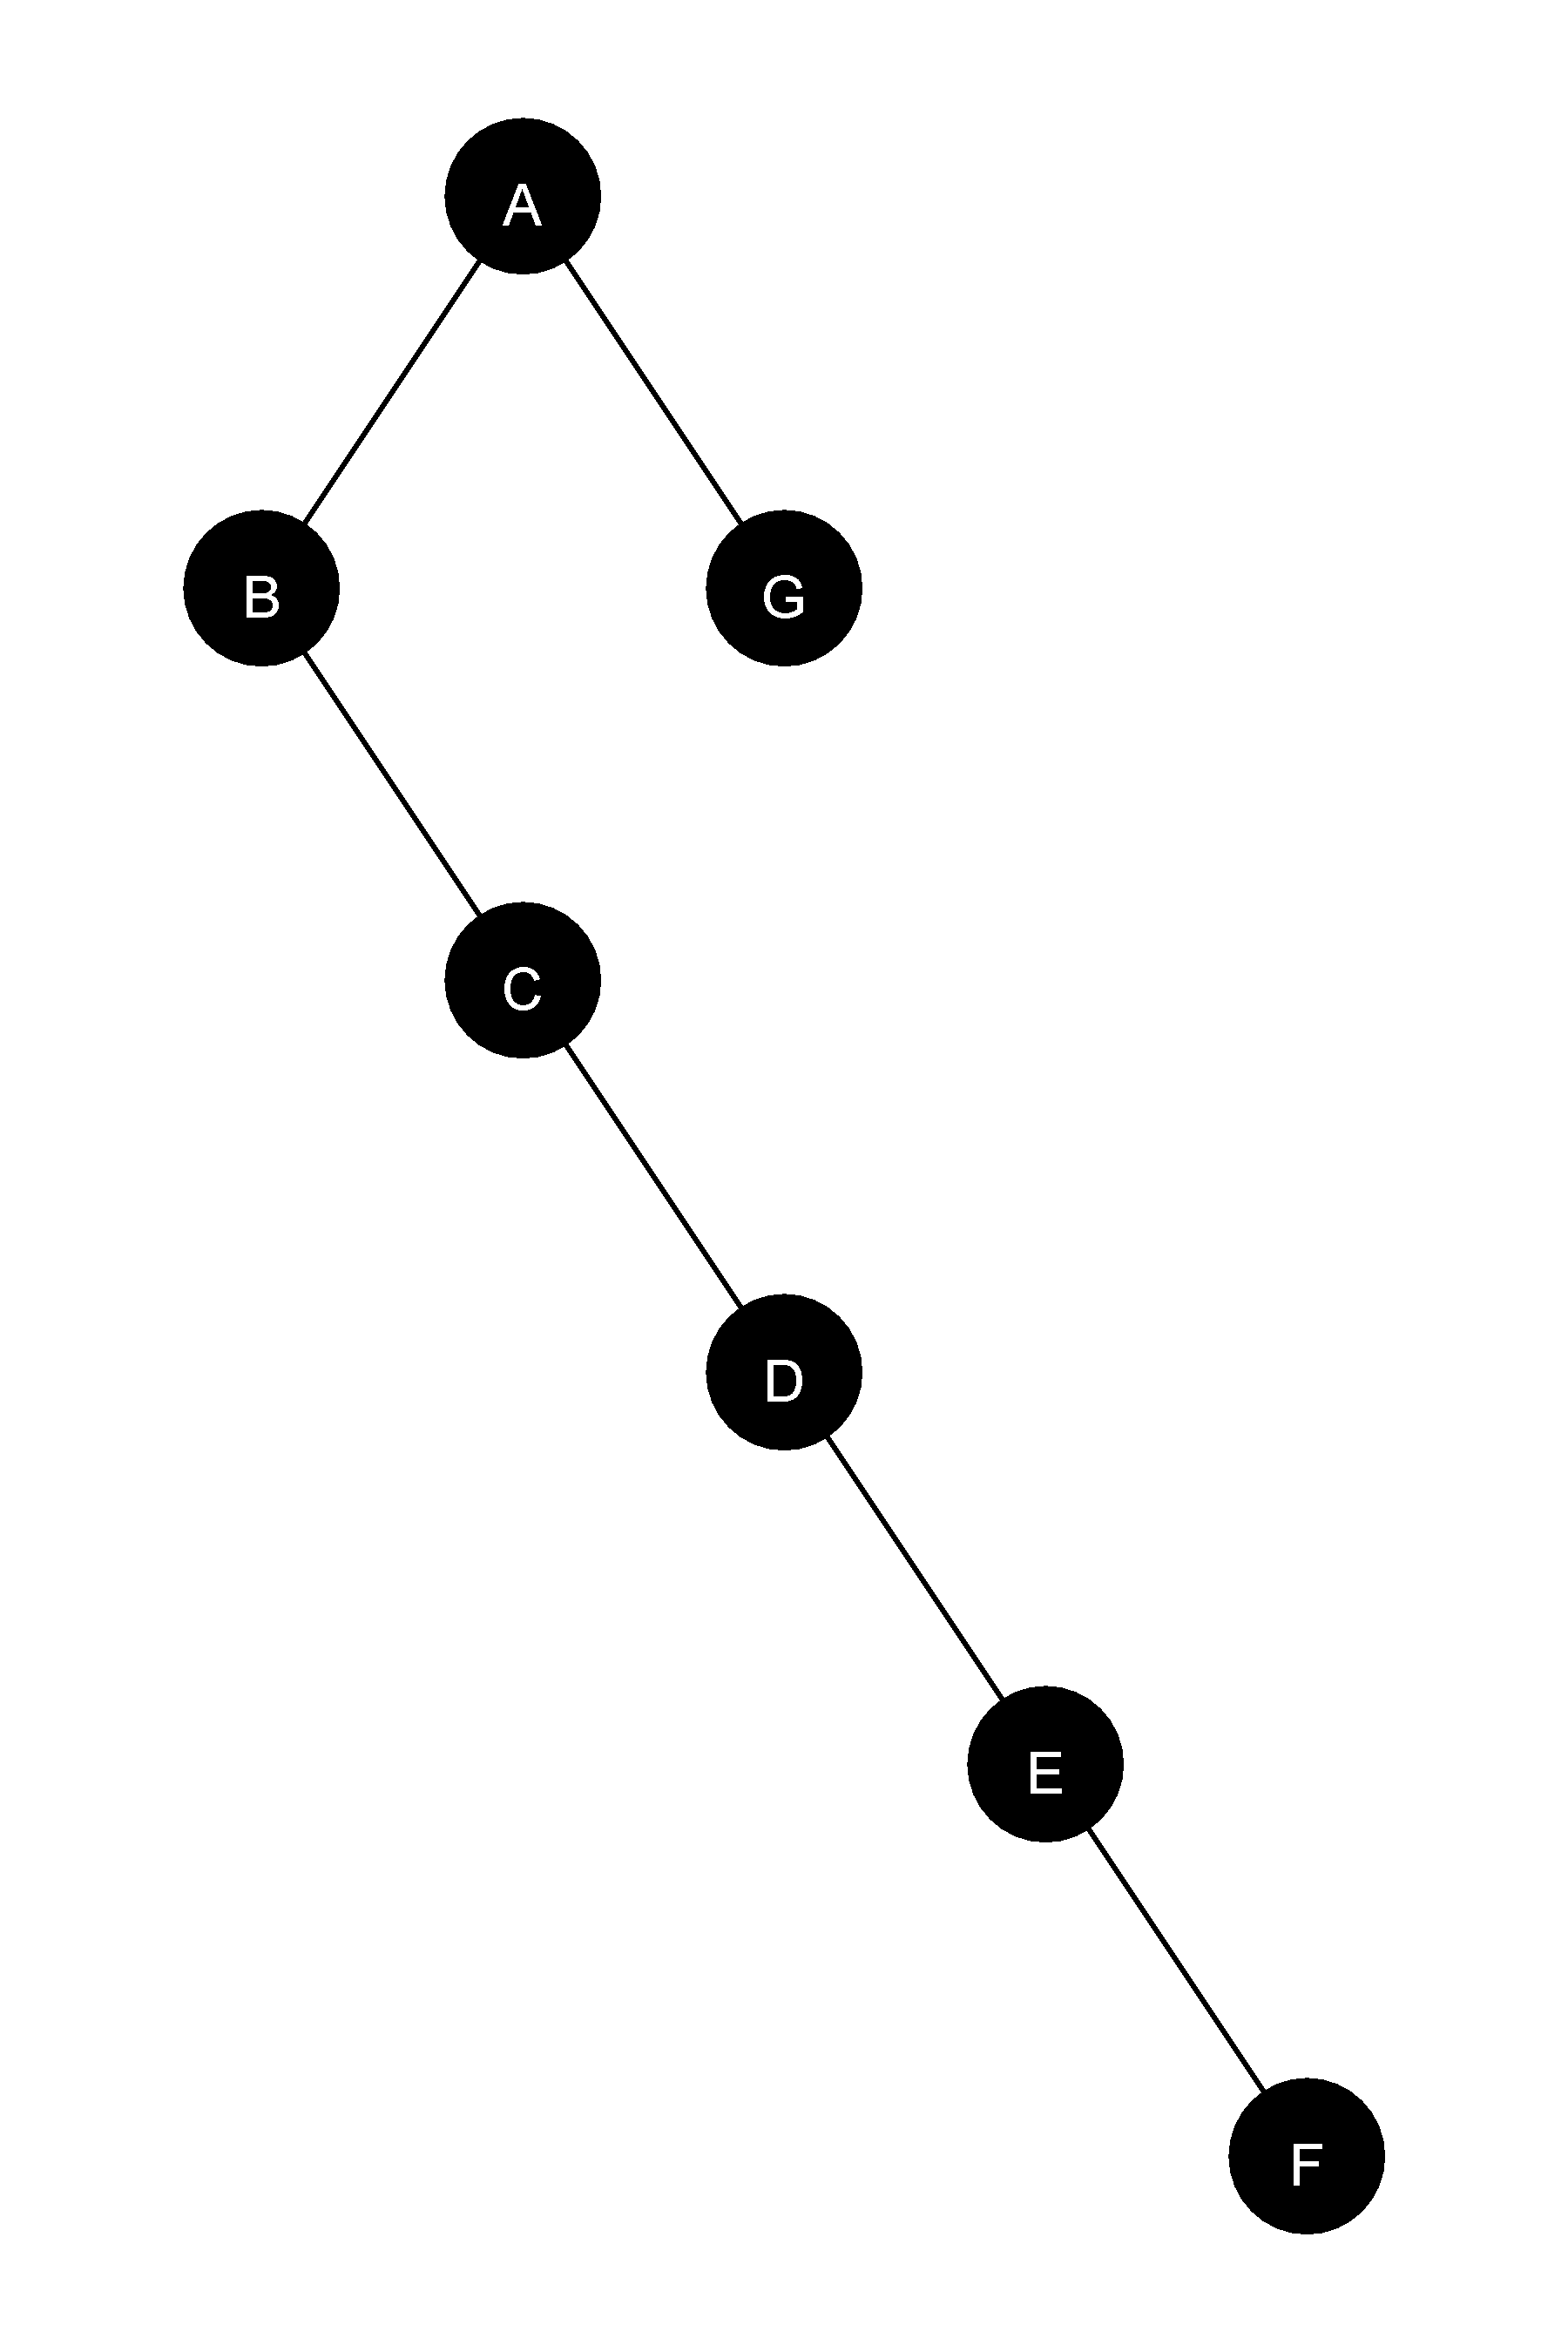
\includegraphics[scale = 0.06]{abbildungen/tree_spiegel_1_a2}
    \end{minipage}
    \hfill
    \begin{minipage}[t]{0.45\linewidth}
        \centering
        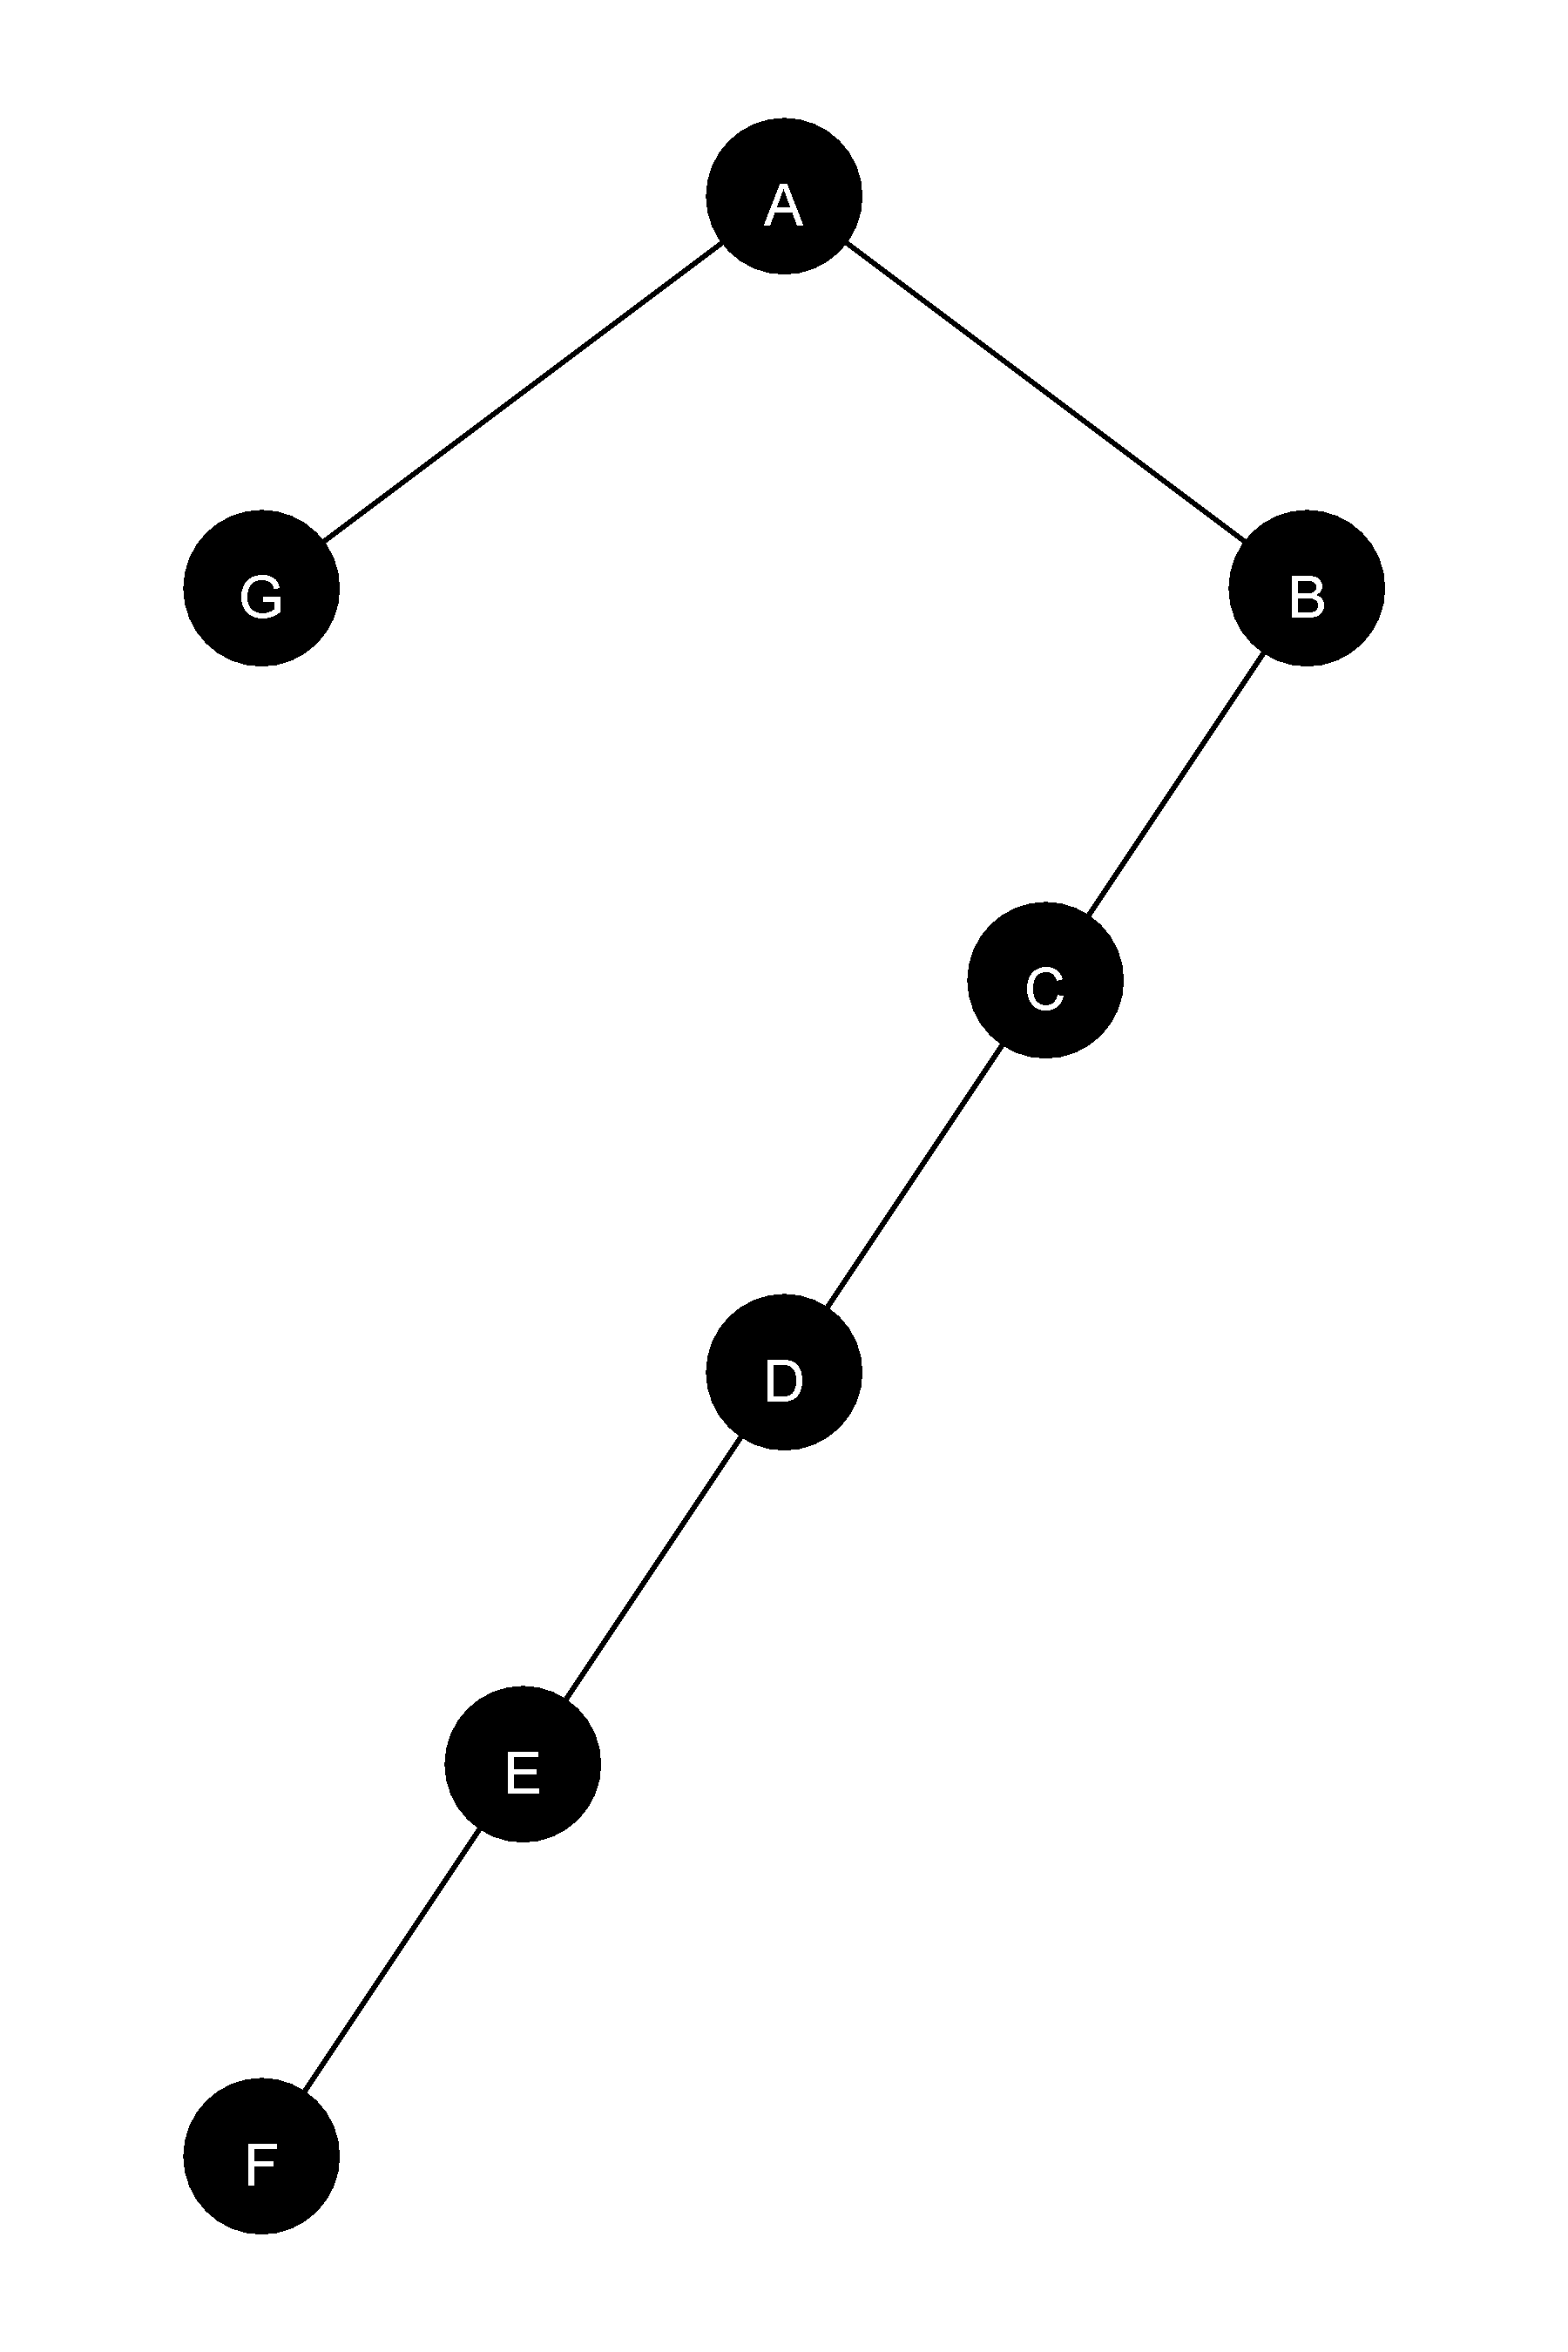
\includegraphics[scale = 0.06]{abbildungen/tree_spiegel_2_a2}
    \end{minipage} 
    \caption[]{Baum und Spiegelung gezeichnet nach WS}
    \label{pic:WS_Spiegel}
\end{figure}

\begin{figure}[ht]
    \centering
    \begin{minipage}[t]{0.45\linewidth}
        \centering
        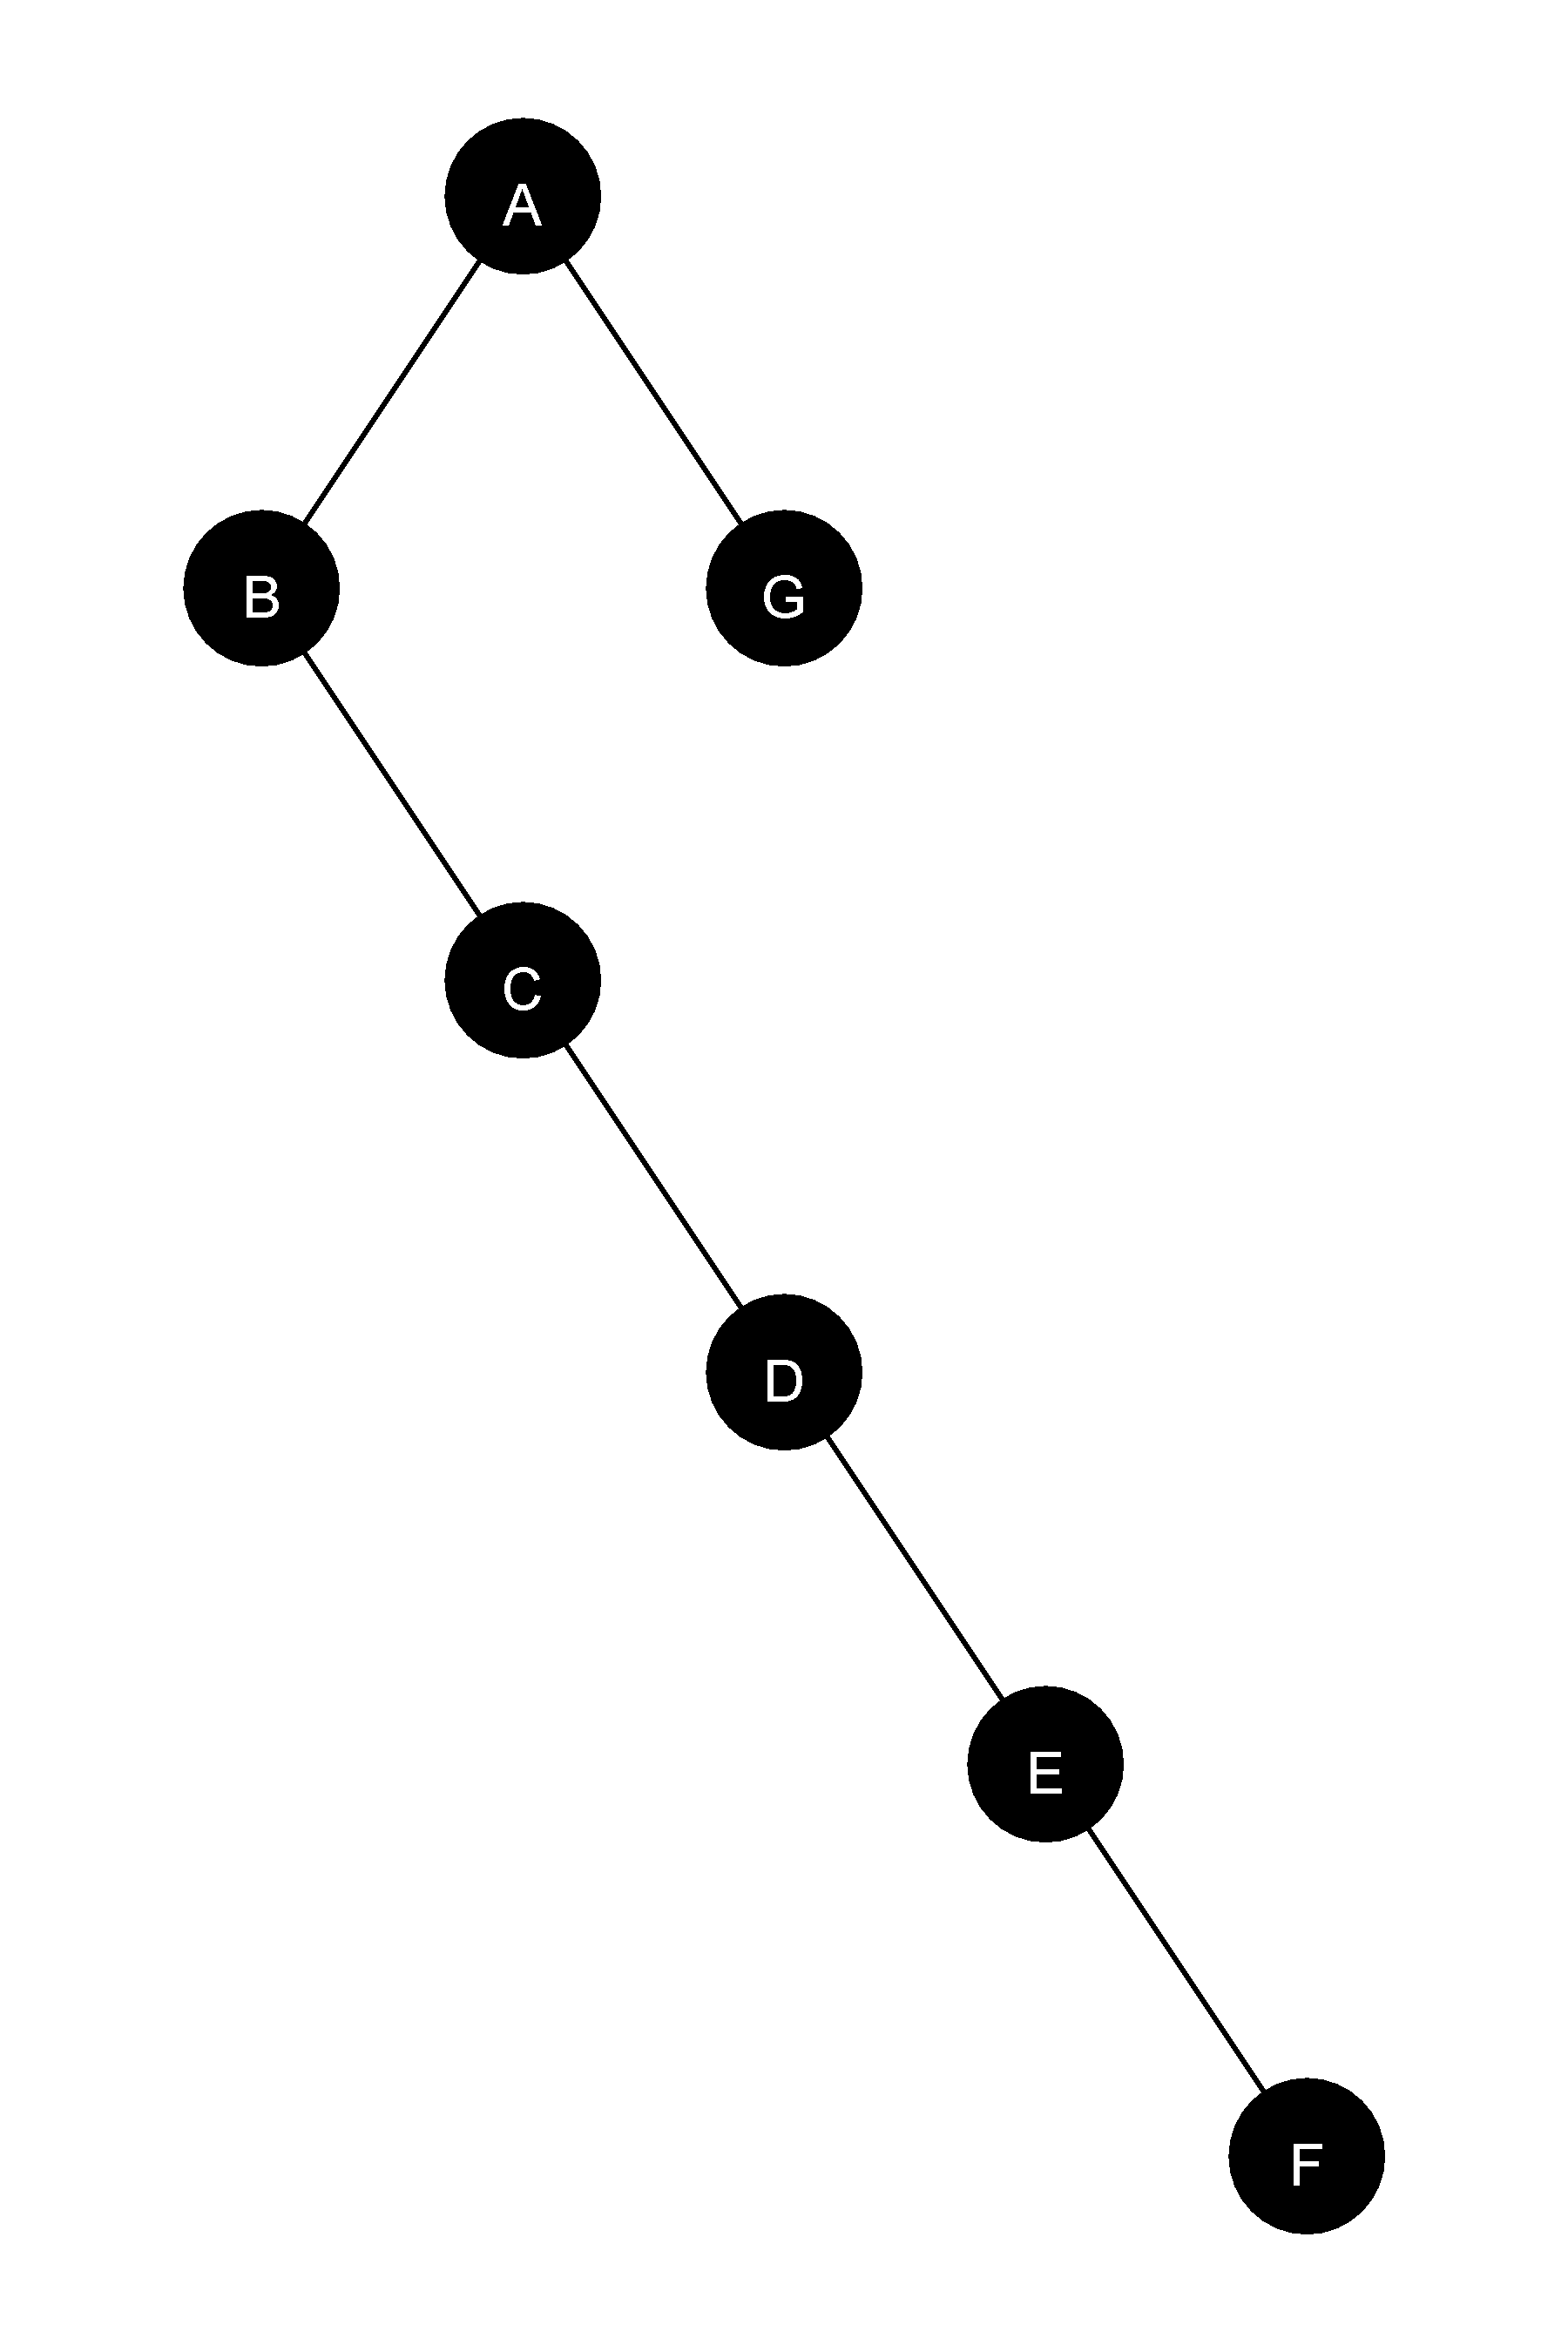
\includegraphics[scale = 0.06]{abbildungen/tree_spiegel_1_a3}
    \end{minipage}
    \hfill
    \begin{minipage}[t]{0.45\linewidth}
        \centering
        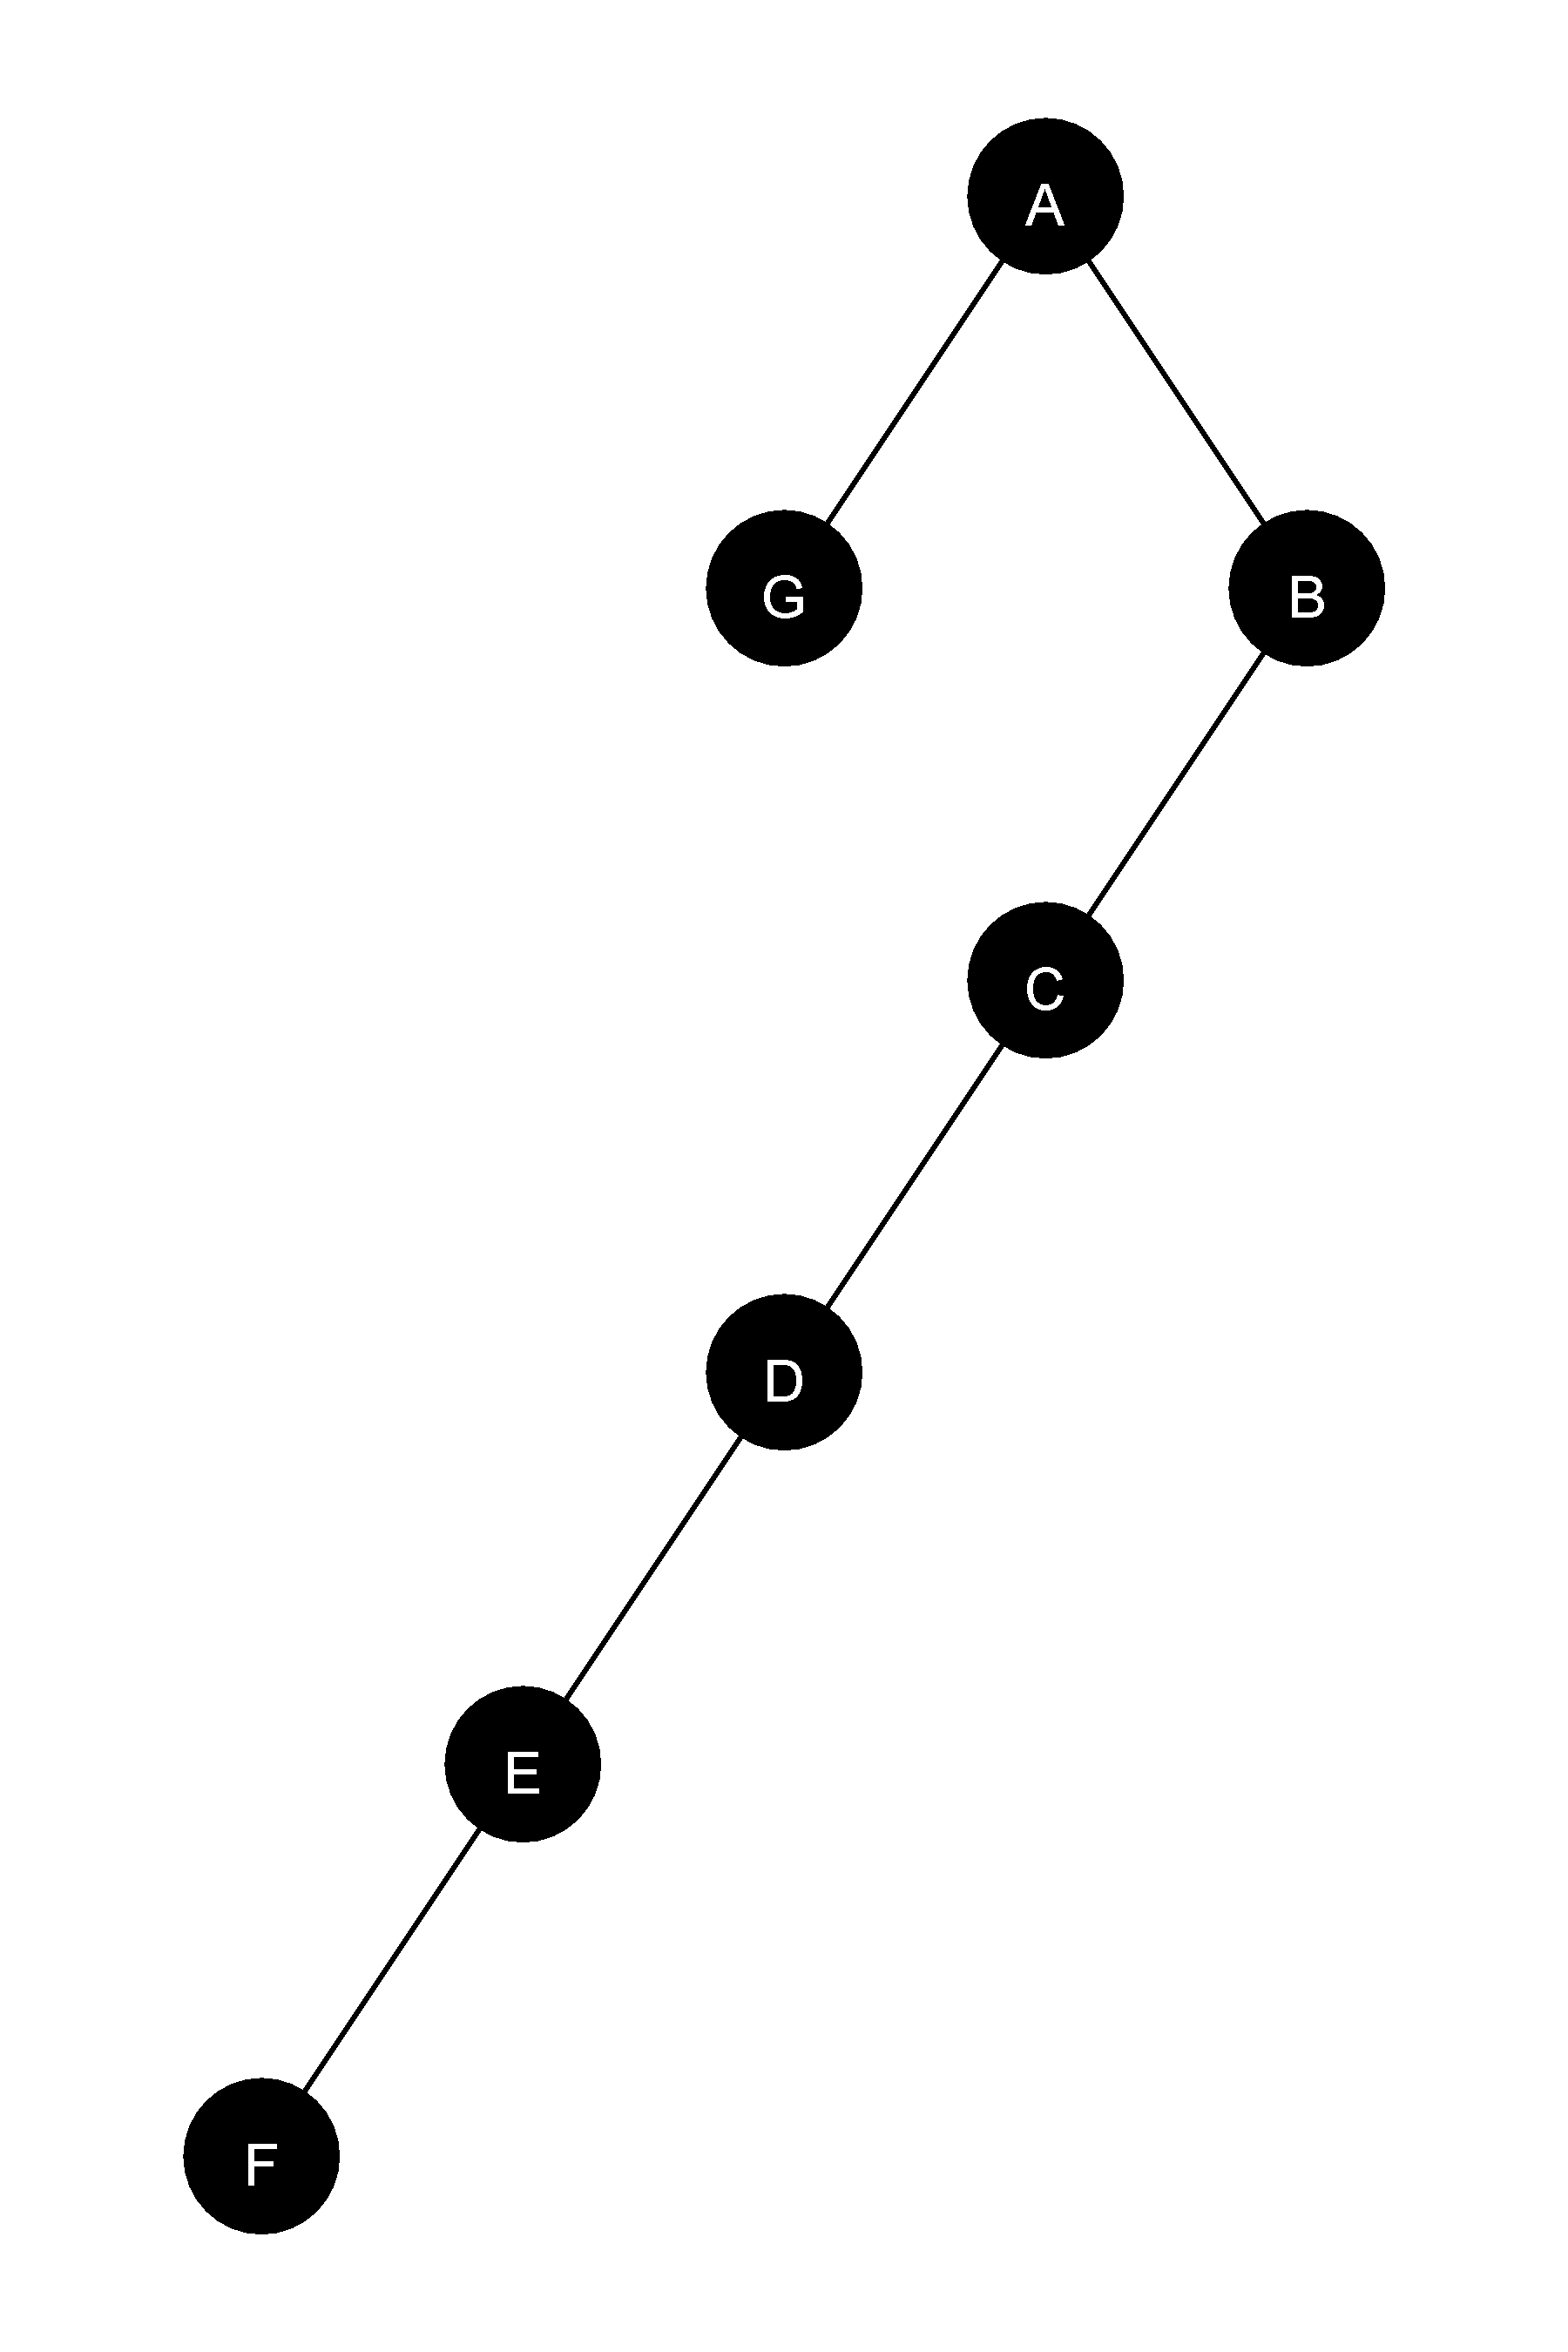
\includegraphics[scale = 0.06]{abbildungen/tree_spiegel_2_a3}   
    \end{minipage}  
    \caption[]{Baum und Spiegelung gezeichnet nach TR}
    \label{pic:TR_Spiegel}
\end{figure}

\chapter{Anhang B}
\label{chap:anhang_b}

\lstinputlisting[caption={Knoten-Klasse}]{abbildungen/git/src/algos/Knoten.java}

\lstinputlisting[caption={Binary-Klasse}]{abbildungen/git/src/algos/BinaryKnoten.java}

\lstinputlisting[caption={WS-Naiver-Algorithmus-Klasse}]{abbildungen/git/src/algos/NaiverAlgorithmus.java}

\lstinputlisting[caption={WS-Algorithmus-Klasse}]{abbildungen/git/src/algos/VerbesserterAlgorithmus.java}

\lstinputlisting[caption={RT-Algorithmus-Klasse}]{abbildungen/git/src/algos/TilfordAlgorithmus.java}

\lstinputlisting[caption={Zusatzklasse: Trees}]{abbildungen/git/src/algos/Trees.java}

\lstinputlisting[caption={Zusatzklasse: Drawer}]{abbildungen/git/src/algos/Drawer.java}

\lstinputlisting[caption={Zusatzklasse: Mains}]{abbildungen/git/src/algos/Mains.java}

% ***************************** BACK MATTER ***********************************
%\thispagestyle{empty}

%\addcontentsline{toc}{chapter}{\protect\numberline{}Eidesstattliche Erklärung}
%\chapter*{}
\vspace*{0.5cm}
\noindent

Hiermit versicheren wir, dass wir die vorliegende Arbeit selbstständig verfasst und keine anderen als die angegebenen Quellen und Hilfsmittel benutzt haben. Wir versicheren, dass wir alle wörtlich oder sinngemäß aus anderen Werken übernommenen Aussagen als solche gekennzeichnet haben, und dass die eingereichte Arbeit weder vollständig noch in wesentlichen Teilen Gegenstand eines anderen Prüfungsverfahrens gewesen ist.

\vspace{3cm}
\toponym, den \today

\end{document}